\documentclass[6pt]{article}
\usepackage{geometry}                % See geometry.pdf to learn the layout options. There are lots.
\geometry{letterpaper}                   % ... or a4paper or a5paper or ... 
%\geometry{landscape}                % Activate for for rotated page geometry
%\usepackage[parfill]{parskip}    % Activate to begin paragraphs with an empty line rather than an indent
\usepackage{graphicx}
\usepackage{amssymb}
\usepackage{epstopdf}
\usepackage{tipa}
\usepackage{amsmath}
\usepackage{floatrow}
\usepackage{subcaption}
\usepackage{apacite}
\usepackage[]{natbib}

\DeclareGraphicsRule{.tif}{png}{.png}{`convert #1 `dirname #1`/`basename #1 .tif`.png}
\graphicspath{{/Users/marlon/Documents/BA/thesis/pictures/}}

\title{Unsupervised Cognate Identification with Variational Autoencoders}
\author{Marlon Betz}
%\date{}                                           % Activate to display a given date or no date

\begin{document}
\maketitle
\newpage
\tableofcontents
\newpage

\section{Introduction}

Historical Linguistics investigates language from a diachronic perspective, i.e. it seeks to uncover the history of languages and the structure of the hidden forces that drive language change.  Computational Historical Linguistics accordingly deals with computational methods to explore the history of languages and topics closely related to it, such as phylogenetic inferences of language families \citep{bouckaert2012mapping}, migration of language speakers \citep{gray2009language}, inferring lexical flows between languages \citep{dellert2015uralic} or modeling sound change \citep{bouchard2013automated}.  
On the other hand, deep neural networks have been proven to uncover latent features of data and use them for a variety of tasks, such as computer vision or various NLP tasks, e.g. Statistical Machine Translation \citep{zhang2014bilingually,lauly2014autoencoder}, Paraphrase Detection \citep{socher2011dynamic}, Sentiment Analysis \citep{socher2013recursive} or Speech synthesis  and recognition \citep{hinton2012deep,zen2014deep}. 
Moreover, bayesian inference models have been proven to allow for a detailed analysis of data and testing hypotheses in various fields of Computational Linguistics \citep{crocker2010computational,chater2006probabilistic}, while for instance in the form of Latent Dirichlet Allocations they provide a strong tool for document classification systems \citep{blei2003latent}. In fact, Bayesian models build the backbone for most current phylogenetic surveys \citep{gray2009language,bouckaert2012mapping,bouchard2013automated}.
Over the past few years, deep neural networks have been interconnected with Bayesian methods in the form of Deep Generative Models. They combine the strength of deep networks to uncover latent features with the power of bayesian inference. Today, deep generative models are the main object of current AI research \citep[p. 654]{Goodfellow-et-al-2016-Book}. 
 However, Computational Historical Linguistics has hardly been touched yet by the current Deep Learning boom (a notable exception is \cite{rama2016siamese}). 
 In fact, most computational models here are either adaptations or direct copies of those used for the description of biological data. 


In this thesis, I will propose a novel view on cognate identification as latent representation learning \citep{bengio2013representation,Goodfellow-et-al-2016-Book}. Coming from the idea that certain computer vision models are shown to generalize well how to rotate a three-dimensional object in an two-dimensional projection and to find latent linear dependencies between high-level features \citep{radford2015unsupervised,dosovitskiy2015learning}, this thesis proposes a model that treats cognates as the same latent objects just seen from the perspective of another language. Sound changes, as realization of such changed perspectives, can be described as linear dependencies over words embedded in a latent space. Here, differences in the actual phonological realization of a word only blur the underlying latent structure of it, which can be shared with other words that are etymologically related. That latent structure is sampled from a simple bayesian hierarchical model, which allows for bayesian inference modeling, such as setting a prior belief on what such a latent structure should look like. The model described here is relatively simple, as it is a direct adaptation of Variational Autoencoders \citep{kingma2013auto}, a quite recent deep generative architecture that combines non-linear dimensionality reduction with the strength of variational bayesian inference. However, it can be used as a basis for more detailed research on how language change can be model with deep learning tools. 


I will first start by giving an overview of the problem of cognate identification and related fields of research. I will give a background on why cognate identification is important to discuss the historical connections between languages and further provide an overview on several established methods to detect cognates.  Then I will proceed to explain the motivations why variational autoencoders are helpful tools for cognate identification and modeling sound change in general. I will then discuss the actual architecture of the inference model. This first covers a general overview on the components included in the model. I will then in detail look over all components in particular. This will first cover a discussion of different methods of phoneme vectorizations. This is followed by a general overview on autoencoders as non-linear dimensionality reduction architectures first and then a description of variational autoencoders in particular, which build the basis for the model described here. I then come to the discussion how to cluster the words, i.e. to assign the actual inferred cognacy labels. Then I will document how well those methods can be used to infer cognacy between words. I will compare the inferred labels with expert judgements first and then see how the inferred labels can infer language phylogenies, using both neighbor joining and established bayesian models of cognate evolution. Finally, I will give a resume on the model described here.


\section{Motivation}
\label{Motivation}
\begin{figure}[h]
\begin{center}
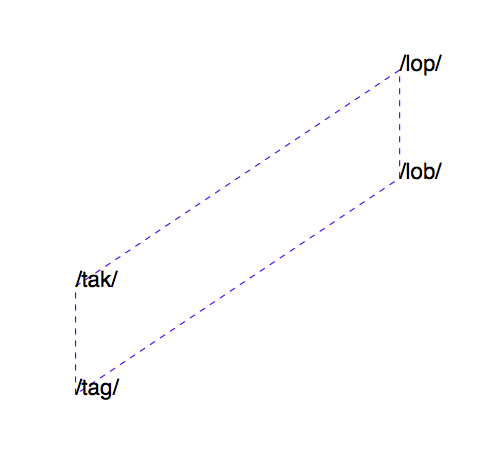
\includegraphics[width=0.5\textwidth]{sc_fake_example} 
\caption{Visualization of the concept of sound change as a walk in latent space. Here, sound changes are vectors from one word to another, where both word forms are given as points in latent space. The vector from /lob/ to /lop/ would be the same as from /tag/ to /tak/, as both vectors would describe the loss of voice in the word-final phoneme. This linear dependence means that if we fit a regression model from /tag/ to /tak/, we could generalize well to predict /lop/ from /lob/. The different lengths of the vectors are than proportional to probabilities of such as sound change to appear. Here, final devoicing should be more probable than a change from /lop/ to /tak/. }
\label{fig:final_devoicing}
\end{center}
\end{figure}

Finding words across different languages that share some common historic origin is one of the most important tasks of Historical Linguistics. If languages share vocabulary, their speakers should also share some common historic origin. Estimating the historical evolution of languages with phylogenetic algorithms presupposes knowledge if certain words are related or not. 


The task of manual cognate identification is usually connected to the \textit{comparative method}. Here, one starts by looking for words that share roughly the same meaning and phonological shape. Then, the actual phonemes are compared to each other to find sound correspondences between languages. Taking phonological universals into account, one can then start to derive some phonemes from others, or estimate some common predecessor for those phonemes compared to each other. In that way, one can reconstruct proto-forms of words. Then, one has to check if the phonological system of such reconstructed vocabularies obeys phonological universals. If that should be the case, one repeats all the steps before with some finer grained analysis, to look for more subtle phonological changes
 for certain words until several words can be derived from one inferred proto-form, and hence can be called cognates\citep[p. 191]{trask1996historical}.  
 

In linguistic literature, such estimated sound changes from one ancient form to a recent one are usually described as a change of distinctive phonological features over phonological symbols. For instance, a sound change such as final devoicing as in Middle High German /h\textipa{U}nd/ $\rightarrow$ New High German /h\textipa{U}nt/ "dog" would be captured by an string edit rule like
\begin{equation}
/d/ \rightarrow /t/ / \_ \#
\label{eq:final_devoicing_symbolic}
\end{equation}

that says that /d/ becomes /t/ before the end of a word. Usually, such sound changes are shown not to appear randomly, but to co-occur according to some latent features. E.g. a sound change like above should leave the language without final /d/, while final /b/ and /g/ would be allowed. Such situations are evolutionary highly unstable, so we would expect the other voiced plosives to change to /p/ and /k/ accordingly. This is due to latent phonological features such as \textsc{[voice]}, \textsc{[labial]} or \textsc{[ATR]}, which are usually described to appear either in a binary or privative feature space \citep{chomsky1968sound}. Accordingly, our rule from above could be generalized to

\begin{equation}
\textsc{[+voice]} \rightarrow \textsc{[-voice]} / \_ \#
\label{eq:final_devoicing}
\end{equation}
which describes the loss of voice at the end of a word.

However, this method is painstaking if the number of languages and words to compare increases. Hence, computational models that perform cognate identification are needed to explore the vastness of languages that are still uncategorized or where family topologies are disputable.

Computational models of sound change usually treat words as string of symbols and sound change as substitution of substrings. This follows the idea that sound changes can be modeled by context-sensitive rules like in Eq. \ref{eq:final_devoicing_symbolic}. \cite{bouchard2007probabilistic,bouchard2013automated} use a generative model that learns to substitute substrings in some latent order and achieve good performances on the reconstruction of ancient forms of words as well as on cognate identification. However, such a method has two major drawbacks: On the one hand, it specifically needs the topology of the languages phylogeny to be known beforehand. This problem does not exist for certain language families with established tree topologies, but can be problematic if language relationships are not totally clear. On the other hand, such purely symbolic models need lot of data to generalize well. \cite{bouchard2007probabilistic} for example underline that their model cannot model chain shifts as such.

To counter those problems, this thesis proposes a novel model of of sound change under the following assumptions:
\begin{enumerate}
\item Phonemes and words cannot only be compared according to some distance metric, but moreover are situated in some latent space that is the underlying causal factor for that distance metric. Certain subspaces of that latent space encodes some latent information of the words embedded in that subspace, but moreover encodes information for similar words that \textit{could} be embedded there, but are not found in the data as such. This also means that functions connecting our data with that latent space should be smooth. 
%This allows the model to group certain data points together if they behave in some similar way and further allows the model to generalize from training examples to nearby points in input space, even if they were not trained on. 
This smoothness assumption builds the basis for several machine learning algorithms \citep[p. 557]{Goodfellow-et-al-2016-Book}. 
\item The relationships between the data can be explained by some linear function, i.e. the data is linearly dependent. This should allow for good predictions even when the test data is far away from the training data. Again, this assumption is important for several machine learning algorithms, such as Generalized Linear Models \citep[p. 557]{Goodfellow-et-al-2016-Book}.
\item Those underlying linear factors that produce the data are to abstract to see directly, but only exist in some highly-abstract latent space that is not directly visible. This means that some decoder function that links latent representations to the actual data has to be non-linear.
\item The model should be probabilistic, which allows for bayesian inference.  That is, the model generates the latent representation by sampling from some prior or posterior. From this also follows that the model should treat factors that change some latent representation as causes for variation of the actual data, not vice versa \citep[p. 557]{Goodfellow-et-al-2016-Book}.

\end{enumerate}
For the task of cognate identification, the first point is the most important. As it states that cognates, as they are usually expected to have similar shapes, should be clustered in such subspaces, we can use clustering algorithms to assign labels to such cluster. Word embeddings that share such a label can than be interpreted as inferred cognates.
To address the smoothness assumption, we have to make sure that such a model treats phonemes and words not as symbols, but as points or distributions in some latent space. This allows for some tokens to be inherently closer to each other. Section \ref{Phoneme Vectorization} will discuss several such embedding methods for phonemes and section \ref{Word Embeddings} will explore variational autoencoders \citep{kingma2013auto} as the preferred embedding algorithms for words, as they are deep probabilistic architectures that allow for both non-linearity and bayesian inference.


The linearity assumption allows for the generalization over the compositional character of latent features over phonemes and words. For instance, a sound change $sc$ such as the final devoicing in Eq. \ref{eq:final_devoicing} that derives a recent form of word $w_{recent}$ from an ancient form  $w_{ancient}$ should then correspond to a vector $v_{sc}$ in such a way that 
\begin{equation}
\label{eq:sound_change_linear_dependency}
v_{w_{ancient}}+v_{sc} = v_{w_{recent}}
\end{equation}

From this follows that 

\begin{equation}
v_{sc} =  v_{w_{recent}} - v_{w_{ancient}} 
\end{equation}

That is, we can formulate sound changes such as \ref{eq:final_devoicing} without neither the actual sound change nor the conditioning specifying where the sound change should apply, but only the respective words involved.
If we further assume that that sound change affects another word $w'$, we have

\begin{equation}
v_{w_{recent}} - v_{w_{ancient}}  =  v_{w'_{recent}} - v_{w'_{ancient}} 
\end{equation}
which is equivalent to
\begin{equation}
v_{w_{recent}}  =   v_{w_{ancient}}  + (v_{w'_{recent}} - v_{w'_{ancient}}) 
\end{equation}
%If we want to evaluate that latent feature space, we investigate in how far that compositional structure is preserved in our latent space. 
In fact, such analogy tasks can be used as an evaluation method to test whether the learned embedding space encodes the structure expected to be inherently contained in the data \citep{mikolov2013distributed}. For a visualization of this concept, see Fig. \ref{fig:final_devoicing}.
 

\section{Related Research}

Cognate identification systems can be divided into two three major groups. Supervised systems learn from a set of positive and negative examples to differentiate between cognates and unrelated words. The features used to discriminate between those examples are usually some sort of  string comparison metric, such as normalized levenshtein distance, Dice coefficients or  alignment scores based on the Needleman-Wunsch algorithm  \citep{bergsma2007alignment,inkpen2005automatic}, weighted alignments with predefined weights \citep{kondrak2000new} or PMI-weighted alignments \citep{jager2014phylogenetic}. Another approach has been pioneered by \cite{rama2016siamese}, where siamese convolutional networks are used to differentiate between cognates and unrelated words. Unsupervised systems, on the other hand, also employ such string comparisons, but assume that cognates should share similar shapes and hence the distance between them should be low. Hence, after predefining some threshold, words with mutual distances beyond that threshold are labeled as unrelated, while words closer to each other are labeled as cognates.  LexStat, originally proposed in \cite{list2012lexstat}, can be seen as the gold-standard for unsupervised systems. LexStat first converts all phonemes into a list of features, then creates scoring schemes for all language pairs, computes pairwise distances between all words based on those scoring schemes and finally clusters the words. \cite{mackay2005computing,wahle2013alignment} use Pairwise Hidden Markov Models to score distances between words and show good performance.  \cite{wahle2013alignment} also reports improved performance over PMI-weighted Needleman-Wunsch alignment scores, but only tests the model on Germanic data and uses labels provided by LexStat instead of expert judgements as gold standard. Another family of models focus on modeling sound change directly, but can be used for cognate identification. \cite{bouchard2013automated} learns a probabilistic state-transducer to estimate Proto-Austronesian word forms given words from contemporary languages and the already established tree topology of the language family. If the proto-form of two words is the same, they are judged as cognates. Although they report good performance, their approach has not been carried out so far for other families than Austronesian.

\section{Architecture}
Embedding words as sequences of phonemes is similar to embedding sentences as sequences of words. In fact, there are several deep architectures that use sentence or phrase embeddings to encode latent information stored in the respective sequences, where each token in a sequence itself is represented by latent representation of that token rather than by the token itself \citep{kiros2015skip,zhang2014bilingually}.
Inspired by such models, the model described here also shows a modular architecture:
\begin{enumerate}
\item First, the phonemes of every word are embedded in a latent space, where similar phonemes should cluster in similar subspaces of the latent space. This should allow for better generalization of sound correspondences between phonemes of different languages, following the smoothness and linearity assumption from Section \ref{Motivation}. Section \ref{Phoneme Vectorization} will cover this topic.
\item Then, the words as sequences of such phoneme embeddings should themselves be embedded in another latent space, where words with similar shape should cluster among each other.  Again, the main motivation here is smoothness and linearity, which should help to uncover latent features. Moreover, this component contains the actual variational autoencoder, which samples embeddings from a latent variable and transforms them into actual words. This follows the other two motivations - the unidirectionality of causal factors and the overcomplexity over the true underlying factors that produce the data. Section \ref{Word Embeddings} will cover this topic.
\item Finally, the word embeddings are then clustered in such a way that words that appear together in a cluster are assigned a common label, which is then the predicted cognate class.  This follows again the smoothness assumption, as we expect words with similar latent features to cluster among each other. Here, it is important that the number and respective size of cognate classes per semantic concept can vary, so we have to find a way to cluster the words without any preference over the number of clusters or cluster size. Section \ref{Clustering} will cover this topic.
\end{enumerate}
The separation of learning the phoneme embeddings on the one hand and word embeddings on the other has practical reasons. On the one hand, phonemes that are decomposed into latent features should allow for better generalization even if the pool of words to cluster is small. While encoding sequences of word unigrams has been proven to work well with recurrent variational autoencoders \citep{bowman2015generating}, this approach will, however, not be explored in this thesis since such unigram-based models are know to need a vast amount of training data to generalize well. On the other hand, there are several ways of vectorizing phonemes, as described in Section \ref{Phoneme Vectorization}. If we learn them independently of the word embeddings, we can explore the information directly contained in the phonemes as such and discuss benefits and drawbacks for the respective model.

However, sentence encoding models where words embeddings and sentence embeddings are learned jointly are proven to work well \cite{kiros2015skip}, thus models that learn phoneme and word embeddings jointly can nevertheless be the object of future research.


Moreover, we focus on two separate models:
\begin{enumerate}
\item A model that tries to maximize $P(X|z)$, i.e. that learns the manifold creating the words as such. Such as model is pre-trained on a big corpus of phonologically annotated words. Here, the assumption is that given a big corpus that is representative of the data as such, the model will recognize the latent features of \textit{words as such} and can embed them in a meaningful even if it was not trained on them directly. This model will be referred to as VAE-PT.
\item A model that tries to maximize $P(X|z,concept)$, i.e that learns the manifold creating words given the respective semantic concept. Such a model is useful as we are only interested to cluster words given a concept class. Also, this means that we only look for latent features in a given semantic concept, which should allow for finer-grained latent features. This model will be referred to as VAE-C.
\end{enumerate}

The main point of interest for VAE-PT is its ability to discover the latent high-level connections between words. As the training corpus here would be quite big, there are much more words that are not cognate to each other, hence the probability that cognates cluster among each other here is quite low. As we expect that as the training set increases it becomes more representative for words as such, we rather expect that more common syllable structures that are cluster among each other if they are similar, but not necessarily cognates. Here, words are rather expected to be connected through linear dependencies as described in section \ref{Motivation}. Hence, VAE-PT can rather be seen as a "showcase" that exemplifies the strength of deep generative models employed as a basis for modeling sound change. However, we do not assume it works well for clustering cognates as such, at least as long as we use distance or similarity metrics as input for clustering algorithms.
VAE-C, on the other hand, concentrates on distinguishing words that can actually be cognates. Hence, we expect it to work much better for clustering embeddings, as the probability that clusters coincide with true cognate classes is much higher. Following this, linear dependencies play a less important role here, but nevertheless allow insight into the compositionality of the words to cluster.
\subsection{Phoneme Vectorization}
\label{Phoneme Vectorization}
Various computational models of sound change treat phonemes as purely symbolic, which means they are treated as equidistant to each other. While such models can achieve good performance on the task of modeling sound change  \citep{bouchard2007probabilistic,bouchard2013automated}, they cannot generalize to process data they have not seen during training. Such an ability only comes from the \textit{smoothness assumption} that $f(x + \epsilon d) \approx f(x)$ for unit $d$ and some small error $\epsilon$ \citep[p. 555]{Goodfellow-et-al-2016-Book}. This assumption allows a model to generalize from training data to close poinst in input space.  However, as long as phonemes are treated purely as equidistant symbols, any given trainable model should not be able to generalize to process unseen data.
Moreover, it is established knowledge that certain phonemes share binary features such as \textit{[velar]}, \textit{[voice]}  or\textit{[ATR]} \citep{chomsky1968sound}. Such latent features regulate how certain phonemes are distributed among each other - e.g. unvoiced consonants occur in word-final positions more often than voiced consonants. Hence they also influence the diachronic evolution of the phonological shape of a word - if a sound appears in a context that is not typical for its actual distribution, it either makes the context change or it changes itself to adapt to the context. For instance, palatal consonants often palatalize other surrounding consonants, while voiced consonants often devoice word-finally.
Following that observation, there are a few models that use such features to differentiate between phonemes. I will first cover hand-crafted phoneme vectorization models that are commonly found in the field of computational historical linguistics, and then compare those with phoneme embeddings learned on some big corpus.

\subsubsection{Hand-crafted Vectorization Models}

Most hand-crafted vectorization models are used for weighted string alignments. Here, the distance between two phonemes is used yield an alignment score between the phonemes. \cite{dolgopolsky1986probabilistic} proposes a merger of all phonemes into a set of 10 phoneme groups, where transitions between  members of a group are more likely than transitions between members of a single group. The groupings are based on an analysis of sound-correspondences between 400 languages of northern Eurasia (cf. \cite[p. 119]{list2012lexstat}). For instance, /k/ and /\textipa{\t{tS}}/ are both represented as a symbol K, since /k/ often evolves into /\textipa{\t{tS}}/, for instance in German /\textipa{k\super{h}e:z@}/ and English /\textipa{\t{tS}i:z}/ "cheese". This system has been used by several studies dealing with stochastical aspects of genetic relationships between languages \citep{baxter2000beyond,mortarino2009improved,turchin2010analyzing}. SCA, as an enhanced version of this system that is extended to cover all IPA characters and its most common diacritics as well as vowels builds the basis for LexStat \citep{list2012sca,list2012lexstat}. To turn those sound classes into vectors that can be used as input for the variational autoencoder, each sound class is represented as a binary one-hot vector. While such pooling methods do not necessarily obey the smoothness assumption, they still allow for some phonemes to be closer (i.e. equal) to each other than to other phonemes. 

 \cite{kondrak2000new} further uses 12 real-valued features bounded between zero and one to allow for a weighted alignment of phoneme sequences. Here it is argued that binary features cannot capture the actual continuum e.g. between velar and uvular sounds. Each feature can moreover be weighted to allow for modeling the relative importance of a given feature.


\cite{rama2016siamese}, on the other hand,  uses binary features that are adapted to the ASJP phonemic alphabet (cf. \cite{wichmann2010asjp}). ASJP does not always distinguish certain features for all phonemes. For instance, voice is distinguished for labial fricatives, but not for dental ones. ASJP further merges all clicks. Vowels are differentiated, but only for 5 prototypes. The whole ASJP phoneme set can be found in the appendix. \cite{rama2016siamese} further merges all coarticulations and vowels, as they tend to be diachronically unstable \citep{kessler2007word}, and yields phonemes with 16 binary features each. \cite{rama2016siamese} reports superior performance using those features as a basis for word vectorizations to find cognates with siamese convolutional networks.
\subsubsection{Phoneme embeddings}
\label{Phoneme embeddings}



If we assume that phonemes do not change unconditionally nor randomly, but instead only change distinctive features given the context, it should be able to embed phonemes in a latent space where local subspaces contain clusters of phonemes that appear in similar environments. For instance, if we have the two Italian-Spanish word pairs /\textipa{\t{tS}EntO}/ - /\textipa{T\textsubarch{i}ento}/ "hundred" and  /\textipa{\t{tS}ElO}/ - /\textipa{T\textsubarch{i}elo}/ "sky", we see that /\textipa{\t{tS}}/ appears in a similar context as /\textipa{T\textsubarch{i}}/. If we should find more such cases in our data, it should be possible to embed them close in some latent space, as we assume that points that are close to each other in the latent space should also show similar behavior in the data space. In fact, /\textipa{\t{tS}}/ and /\textipa{T\textsubarch{i}}/ are renderings of a common Vulgar Latin /\textipa{k\textsubarch{i}}/ - hence we can assume that phonemes with similar embeddings share a tendency to develop from one into the other. If we interpret each dimension of an embedding as a value of a latent feature, we expect to yield similar features as those hand-crafted vectorization methods proposed above.



There are several families of algorithms that perform such an embedding. Earlier models are based on factorized co-occurrence matrices, such as Latent Semantic Analysis \citep{landauer2013handbook}. This approach is inherently intuitive, as the factorized context of a given phoneme would then be taken as point in latent space, so similar contexts than inherently lead to proximity in latent space. However, over the past few years, more recent neural embedding models such as word2vec \citep{mikolov2013efficient,mikolov2013distributed,goldberg2014word2vec}  have been shown to outperform those count-based models, although GloVe \citep{pennington2014glove}, as more recent count-based model, seems to achieve similar performance.

Word2vec is a shallow network that consists of a linear encoder and softmax classification layer. There are two architectures: Continuous Bag Of Words (CBOW), that learns to predict a token given its context, and Skip-Gram (SG) that is trained to predict the context given the token. They both have in common that they assume the token and its context to occupy the same location in latent space. This allows for a compositionality of the learned latent features. For instance, to re-use the example from above, the embeddings for /\textipa{T} / and /\textipa{\textsubarch{i}}/ are not expected to be close in the latent space, as the overall contexts they can appear in should be quite different. However, given that they appear together as /\textipa{T\textsubarch{i}}/, the addition or mean of the respective embeddings should be close to each other.

As traditional softmax classification is computaltionally expensive expensive given a larger number of token types, several alternative classifiers have emerged during the past few years. One is Hierarchical Softmax (HS, \cite{morin2005hierarchical}). Here, the classifier layer is a binary tree with the actual token types as leaves. At every node, the network learns to either follow the left or the right branch with a certain probability as in Eq. \ref{eq:hierarchicalsoftmax_nodeprob} that is equal to the sum of the child elements of the respective  branch, but is actually computed as the product of $h^\top$ and the output vector of the word at node $n$ pulled through a logistic sigmoid:

\begin{equation}
p(right|n,c) = \sigma(h^\top v'_n) 
\label{eq:hierarchicalsoftmax_nodeprob}
\end{equation}

This means that in order to calculate the softmax probability of word, we only have to follow the path down to the word leaf instead of summing over all possible token types. For binary trees, this means we only have to pass at most $\log_2(\mid V\mid)$ nodes to calculate the probability of a word, which is a huge performance boost over the traditional softmax classifier. 

Another family of alternative classifiers use sampling-based approaches. Among them, Negative Sampling (NEG; cf. \cite{goldberg2014word2vec}) is the most popular. NEG is originally derived from Noise Contrastive Estimation (cf. \cite{gutmann2010noise,mnih2012fast}). Instead of a classifier as such, NEG samples random tokens from the available token types and learns to distinguish them from the actual tokens that appear in a context. The loss function would then be

\begin{equation}
J_{\theta}  = - \sum_{w_i \in V} [\log \sigma(h^{\top}v'_w)
+ \sum_{j=1}^{k}\log \sigma(-h^{\top}v'_{\tilde{w}_{ij}})]
\label{eq:neg_sampling_3}
\end{equation}

where $k$ is the number of sampled tokens and $v'_{\tilde{w}_{ij}}$ the vector representation of such a sampled word.

A first visual inspection shows that the phoneme embeddings indeed capture some latent information (Fig.  \ref{fig:phoneme_embeddings_word2vec_all}). Broader natural classes such as vowels cluster among each other,  clearly differentiated by their type of articulation, such as nasalization or glottalization. In general, sounds that share a common coarticulation are embedded close to each other. Velar and uvular sounds are also closer to nasalized vowels than plain vowels, as both involve an attracted tongue root during production. Less frequent phonemes, however, cannot really be embedded in a meaningful way. In fact, both Spearman and Pearson correlation indices are 0.9, which indicate that the quality of the embeddings is linked to the frequency of the respective phoneme in the data set.

To evaluate further if such data driven phoneme embeddings are able to capture the natural distinction between phoneme classes, a test set over 108 analogy tests was used to conduct a grid search over several word2vec architectures and their parameters. Each such analogy test was of the form

\begin{equation}
v(phoneme_1) + v(phoneme_2) -  v(phoneme_3) \approx v(phoneme_4)
\end{equation} 

where $v(phoneme_1)$ is the vector corresponding to $phoneme_1$ and $v(phoneme_2) - v(phoneme_3)$ can be seen as the latent phonological information available in $phoneme_2$ but not in $phoneme_3$,  while $v(phoneme_1) + v(phoneme_2) -  v(phoneme_3) $ is then this latent phonological information added to $phoneme_1$, which should be close to the vector corresponding to $phoneme_4$. For example, in

\begin{equation}
v(\textbf{/i/} ) + v(\textbf{/u*/} ) -  v(\textbf{/u/} ) \approx v(\textbf{/i*/} )
\end{equation}
$v(\textbf{/u*/} ) -  v(\textbf{/u/} )$ describes a latent feature that should correspond to \textsc{[+nasalized]}, which is then added to the phoneme \textbf{/i/} to yield a nasalized \textbf{/i*/}.
The grid search was conducted over the following parameters:
\begin{itemize}
\item Model architecture: CBOW, SG
\item Classifier: Softmax, negative sampling
\item Embedding dimensions: $[2, 5,10, 20, 50, 100, 150, 200, 400 ]$
\item Context window size: $[1,2,3,4,5,8]$
\item Number of negative samples: $[1,2, ..., 20]$
\end{itemize}
 Each model iterates five times over the corpus, which consists of all words from the ASJP corpus given the language they belong to is neither artificial nor reconstructed. Every word is bracketed by word boundary tokens.


Fig. \ref{fig:phoneme_embeddings_detailed_evaluation_topn1} shows that the quality varies significantly with regards to the articulation type of the phonemes. For pulmonic consonants the models achieve reasonable performance, while for other coarticulation types the performance is quite bad. When following \cite{jager2014phylogenetic,rama2016siamese} and pooling coarticulation types, the models perform much better, for analogies over plosives, while the performance for fricatives has only slightly improved. 


%\begin{figure}[h!] %  figure placement: here, top, bottom, or page
%\begin{center}
%   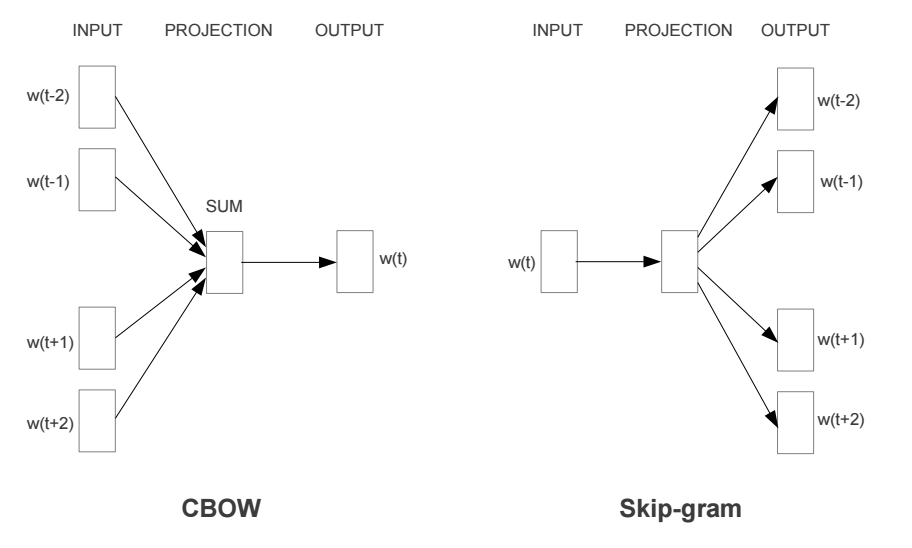
\includegraphics[width=0.75\textwidth]{word2vec} 
%   \caption{The two common architectures of word2vec. The Continuous Bag-of-Words (CBOW) model predicts the current word based on the
%context, and the Skip-gram predicts surrounding words given the current word. From \cite{mikolov2013efficient}.}
%   \label{fig:word2vec}
%   \end{center}
%
%\end{figure}

%
%\begin{figure}[h!]
%\begin{center}
%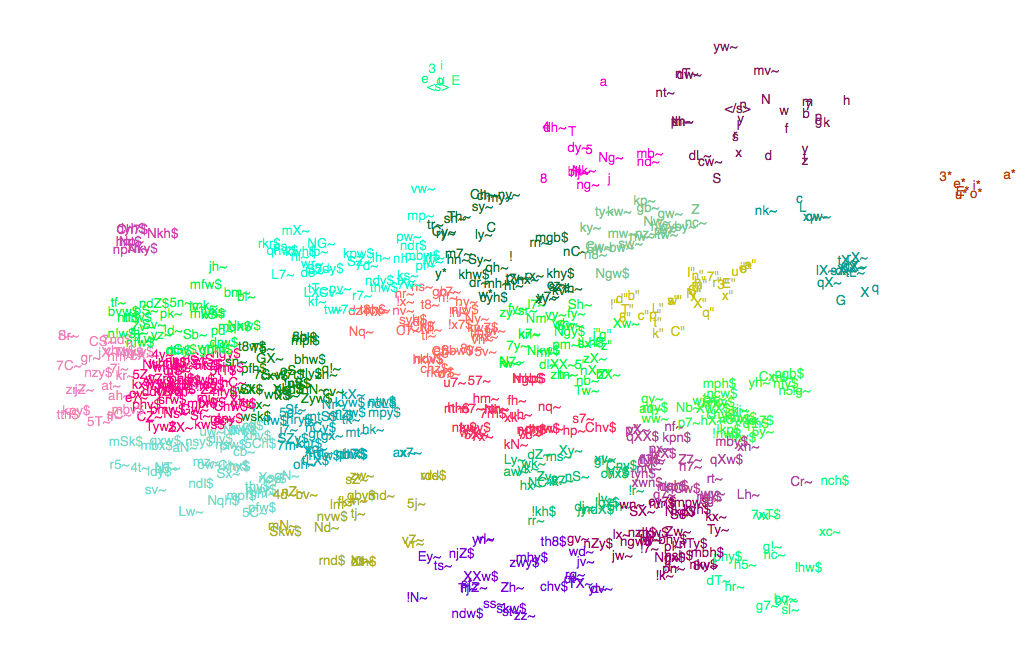
\includegraphics[width=0.5\textwidth]{phoneme_embeddings_overview_ap} 
%\caption{t-SNE visualization of the embeddings of all 720 phonemes contained in ASJP, trained with word2vec. The colors represent clusters inferred by Affinity Propagation. The model can clearly separate vowels and various forms of special articulation types. Pulmonic consonants can also be separated clearly from other coarticulation variants, as can uvular or pre-nasalized sounds. Less frequent phonemes, however, cannot be clearly differentiated. }
%\label{fig:phoneme_embeddings_overview_ap}
%\end{center}
%\end{figure}

\begin{figure}[h!] %  figure placement: here, top, bottom, or page
   \centering
   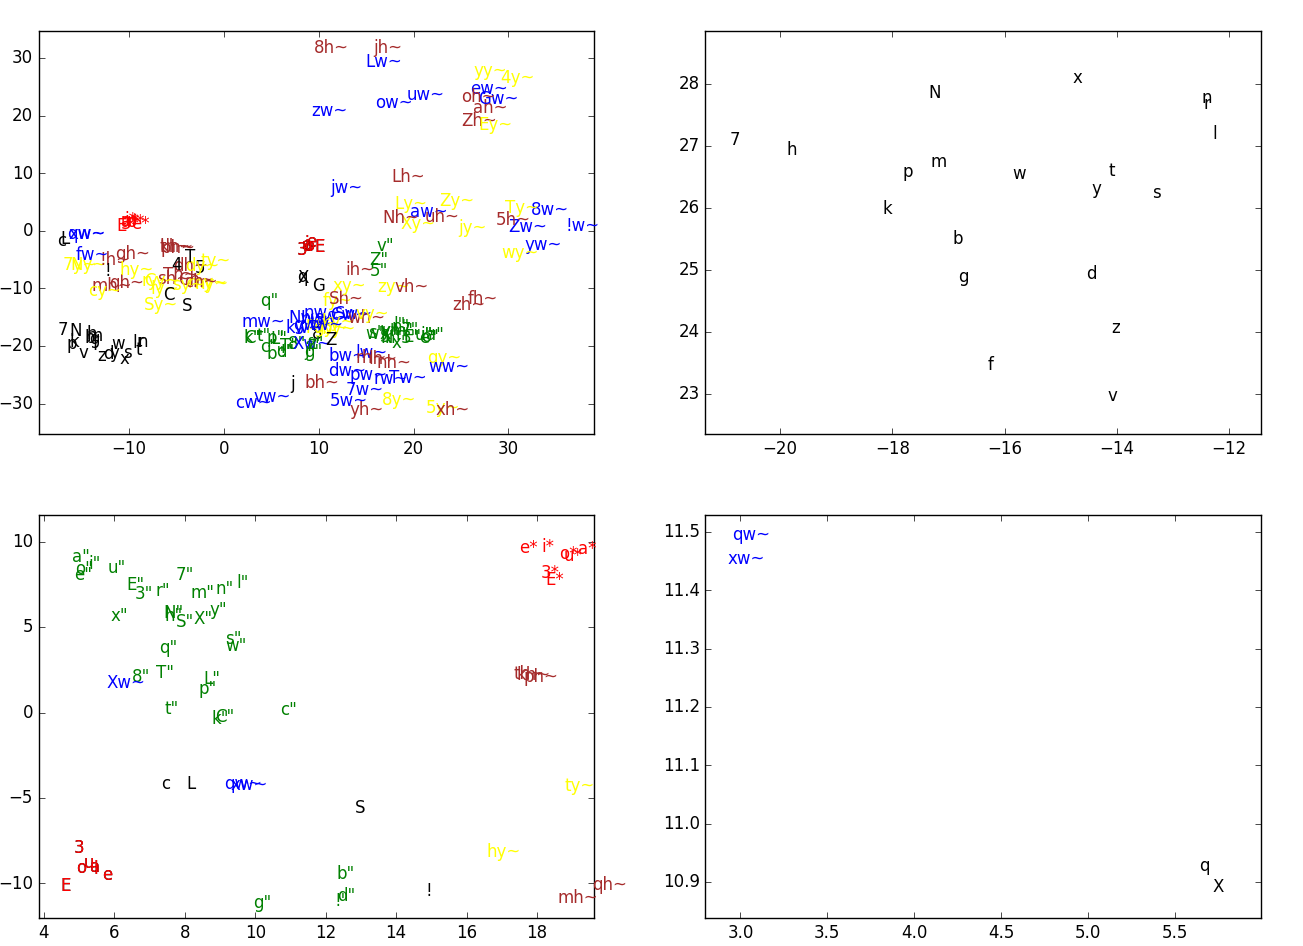
\includegraphics[width=\textwidth]{phoneme_embeddings_word2vec_all} 
   \caption{Some t-SNE visualizations of the embeddings created by word2vec. (top left) The model learns to clearly separate natural classes such as vowels, plain pulmonic or glottalized consonants, while other articulations seem to spread over the feature space. The colors indicate membership of a natural phonological class.  (top right) A more detailed view on plain pulmonic consonants. Note the linear dependencies between voiced and unvoiced plosives and their respective nasal variant. (bottom left) Another detailed view. Note how the labialized uvular sounds cluster among glottalized consonants. (top right) The model seems to capture different manners of articulations across articulation type boundaries, as the linear dependency shows here.}
   \label{fig:phoneme_embeddings_word2vec_all}
\end{figure}

\begin{figure}[h!] %  figure placement: here, top, bottom, or page
   \centering
   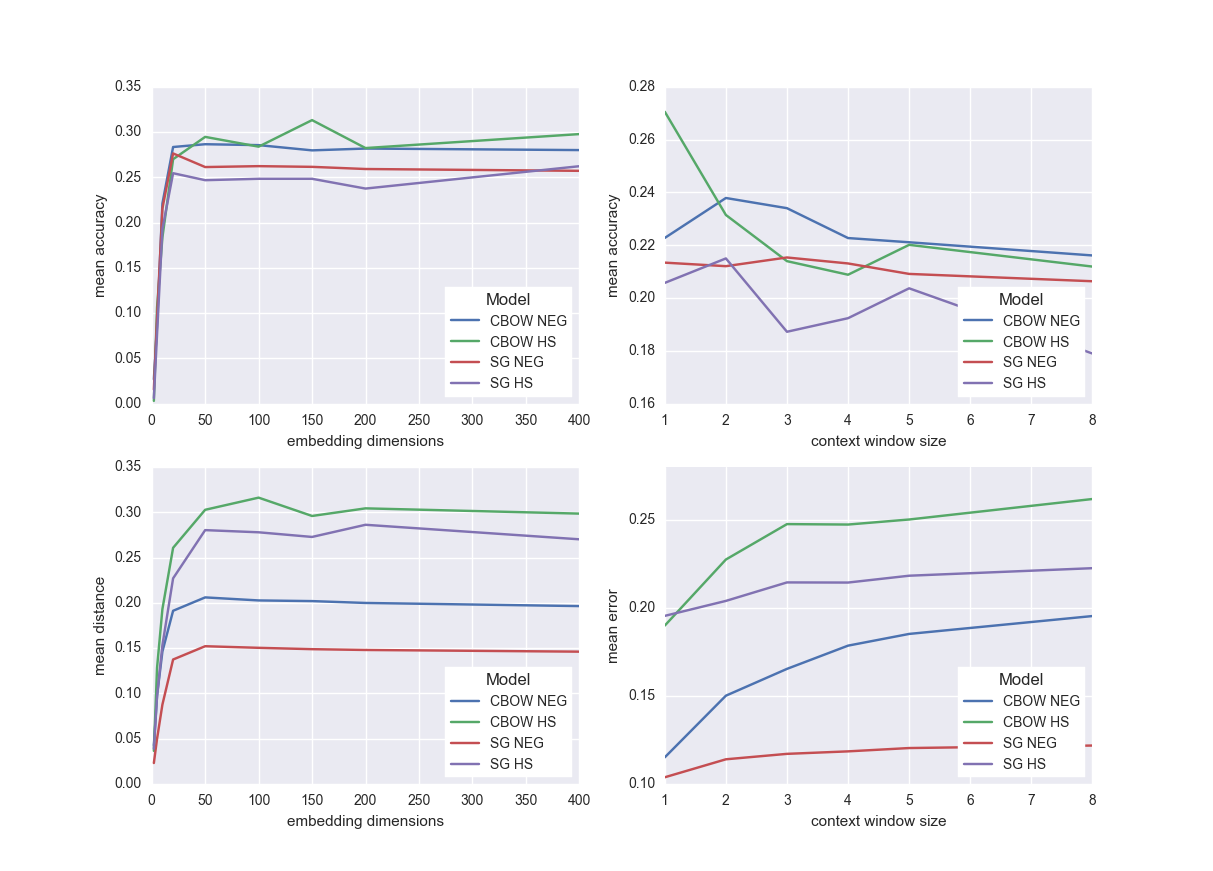
\includegraphics[width=\textwidth]{phoneme_embeddings_4models_comparison_meanAccLossTopn1} 
   \caption{Comparison of the four word2vec models evaluated. (top left) Both CBOW Models perform better than the skip-gram models over all numbers of embedding dimension. (bottom left) Mean distance between the predicted vector and the target with regard to embedding dimensions. Here, negative sampling yields less error than hierarchical softmax. (top right) Mean accuracy for the models with regard to the context window size. The models perform worse the bigger the context is. (bottom right) Mean distance between the predicted vector and the target with regard to context window size. Again, bigger contexts lead to worse predictions. }
   \label{fig:phoneme_embeddings_4models_comparison_meanAccLossTopn1}
\end{figure}

\begin{figure}[h!] %  figure placement: here, top, bottom, or page
   \centering
   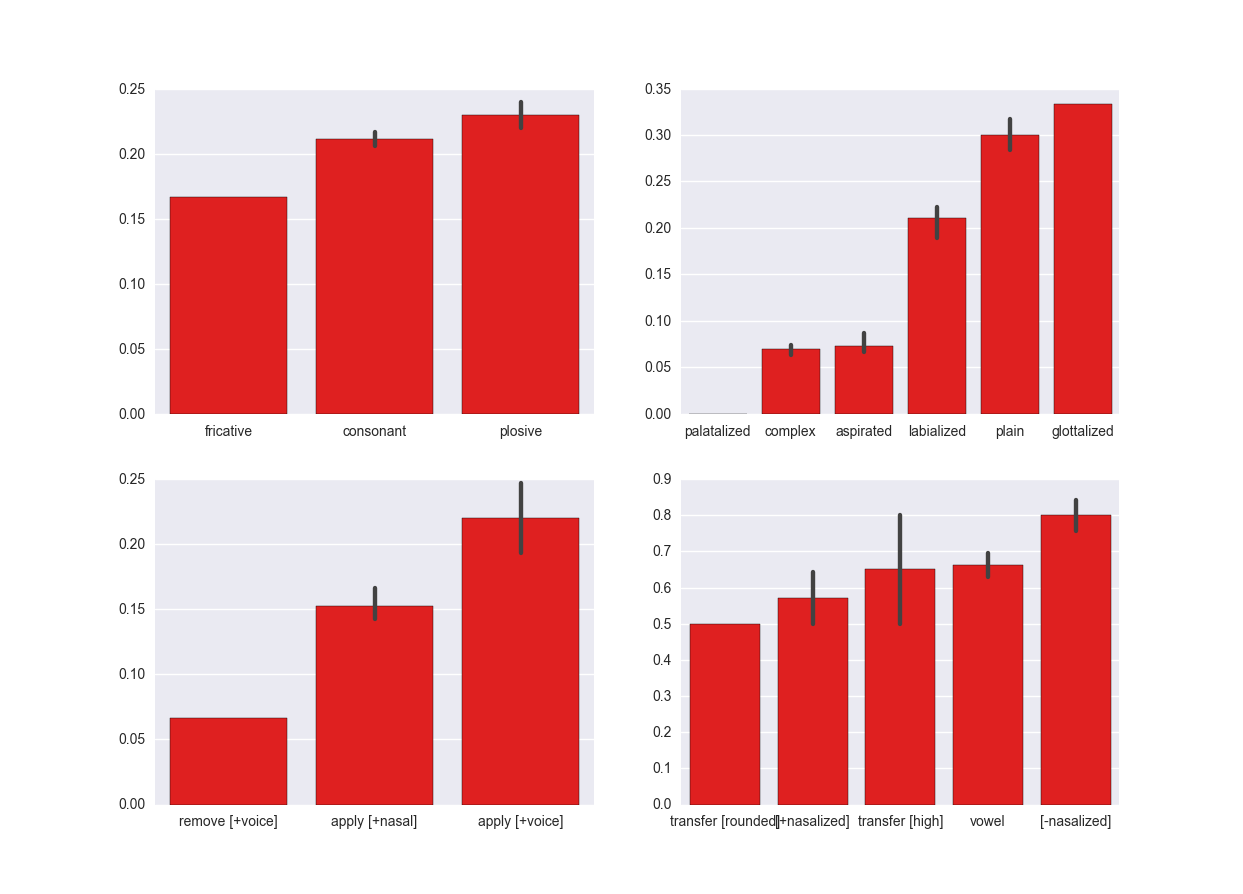
\includegraphics[width=0.75\textwidth]{phoneme_embeddings_detailed_evaluation_topn1} 
   \caption{Mean accuracies for analogies. The model does not seem to be able to capture the compositionality of the latent features too well. (top left) Accuracy is best for plosives across plain pulmonic as well as more complex articulations, while fricatives perform worse. (top right) Glottalized and Plain pulmonic consonant phonemes yield best performance. Among complex articulations, which all perform bad,  labialized phonemes yield best results, while aspirated and palatalized phonemes perform even worse. (bottom left) Adding voice works better than removing it or adding nasality. (bottom right) Vowel analogies work far better than consonant analogies. This should be due to the small number of possible vowel phonemes.}
   \label{fig:phoneme_embeddings_detailed_evaluation_topn1}
\end{figure}

\begin{figure}[h!] %  figure placement: here, top, bottom, or page
   \centering
   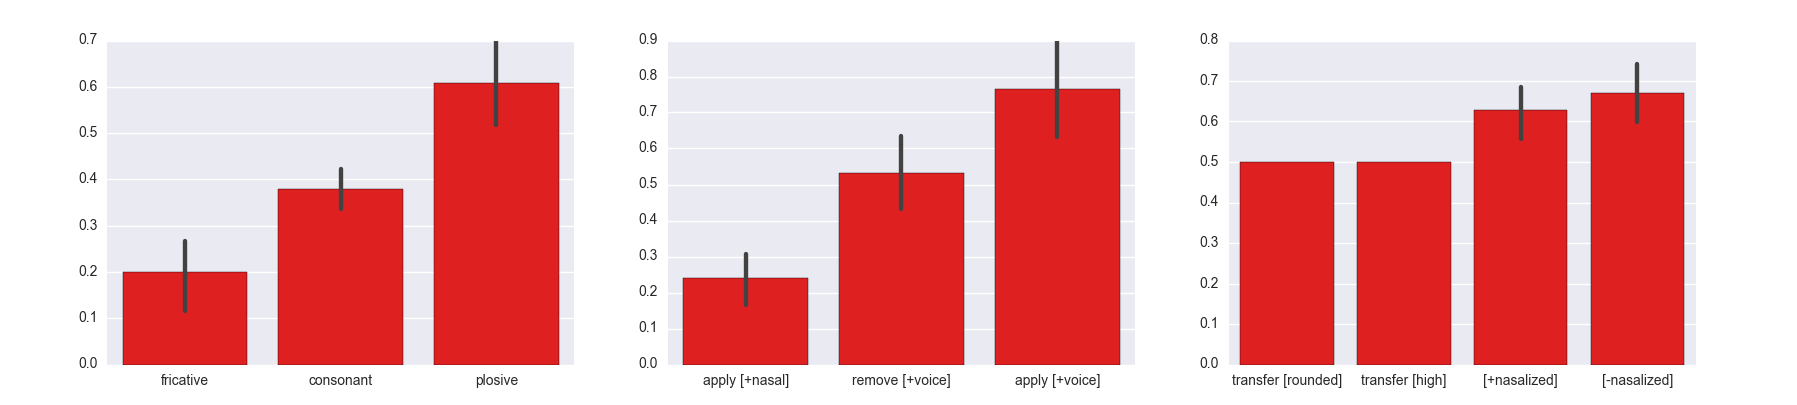
\includegraphics[width=\textwidth]{phoneme_embeddings_detailed_evaluation_consonants_topn1_poooled} 
   \caption{Mean accuracies for analogies over the pooled consonant phonemes. Here, the model is expected to yield better results, as the number of latent features should have been reduced. (left) Accuracy is doubled compared with the unpooled phonemes. (middle) Adding voice works quite well, while removing it still yields acceptable performance. Applying nasality again works quite bad. (right) Vowel analogy tasks seem to work reasonably well, but worse than with unpooled consonants.}
   \label{fig:phoneme_embeddings_detailed_evaluation_topn1_poooled}
\end{figure}


\subsection{Word Embeddings}
\label{Word Embeddings}
\subsubsection{Autoencoders}

Autoencoders are a family of neural network architectures that are trained to construct a code of some given data. Given an encoder function $f: \mathcal{X} \rightarrow \mathcal{Z}$ and a decoder (i.e. generator) function $g: \mathcal{Z} \rightarrow \mathcal{X}$, they are trained on encoding and reconstructing the data, yielding a loss function
\begin{equation}
J(x,g(f(x)))
\end{equation}
 
where $J$ describes some loss function that penalizes the reconstruction error. The dimensionality of $\mathcal{Z}$ is usually assumed to be lower-dimensional, so that autoencoders can be used to reduce the dimensionality of the data, although sparse autoencoders use higher-dimensional hidden layers with some sparsity constraint. If $f$ and $g$ are linear functions, autoencoders are proven to be equal to PCA. If they are non-linear, they allow for the recognition of latent features \citep{hinton2006reducing}. Autoencoders are used in various NLP fields, such as Machine Translation, \citep{lauly2014autoencoder,zhang2014bilingually}, Paraphrase Detection  \citep{socher2011dynamic} or Information Retrieval \citep{silberer2014learning,le2014distributed}. Also, word2vec \citep{mikolov2013efficient,mikolov2013distributed,goldberg2014word2vec} as the probably most popular embedding algorithm is in fact a shallow autoencoder.
\subsubsection{Variational Autoencoders}
\label{Variational Autoencoders}
\begin{figure}[h!] %  figure placement: here, top, bottom, or page
   \centering
   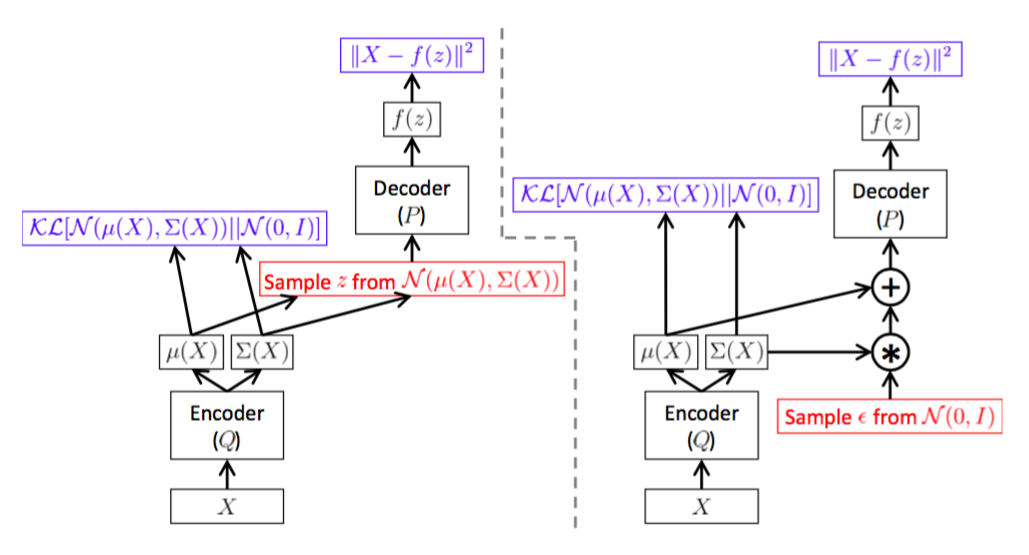
\includegraphics[width=\textwidth]{vae_model_visualization} 
   \caption{Visualization of the Variational autoencoder architecture. (left) The model with original objective as in Eq. \ref{eq:vae_loss_original}. The stochastic unit is inside the network and would not allow for the backpropagation of error gradients through the network. (right) The model after the reparameterization with the objective as in Eq. \ref{eq:vae_loss_reparameterized}. Here, the sampling is interpreted as an input variable, so error gradients can be backpropagated through the whole model. From \cite{doersch2016tutorial}.}
   \label{fig:vae_model_visualization}
\end{figure}

Variational Autoencoders (VAEs) were first described in \cite{kingma2013auto}. Instead of just using a lower-dimensional layer as a bottle neck for non-linear dimensionality reduction, VAEs assume that the code can be modeled by a latent variable $z$ with some prior $p(z)$. This allows for the incorporation of bayesian inference tasks where the marginalization of variables is important, including maximum a posteriori estimates of $\theta$ and an approximation of the posterior $P(z|X)$. Instead of encoder and decoder functions, distributions are used instead to model the relationship between $\mathcal{X} $ and $  \mathcal{Z}$.

As variational models, VAEs do not attempt to sample from the true posterior distribution $P(z|X)$ directly. Popular Markov Chain Monte Carlo methods, such as Gibbs sampling \citep{geman1984stochastic} or Hamiltonian Monte Carlo \citep{duane1987hybrid}, can approximate the true posterior, but rely on whole batches during training, which is not suitable for bigger data sets. Instead, variational method assume that the true posterior can be approximated by another parametric distribution $Q(z|X)$ whose parameters can be estimated analytically. 

In order to approximate the true posterior  $P(z|X)$ with the approximate posterior $Q(z|X)$, we want to minimize the Kullback-Leibler divergence from the true posterior to its approximation: 

\begin{equation}
D_{KL}(Q(z|X)||P(z|X)) = E_{z\sim Q}[\log Q(z|X) - \log P(z|X)]
\end{equation}

Here, we can use Bayes' rule to yield 

\begin{equation}
D_{KL}(Q(z|X)||P(z|X)) = E_{z\sim Q}[\log Q(z|X) - \log P(X|z)-\log P(z)] + \log P(X)
\end{equation}

where $\log P(X)$ is outside the expectation since it is not dependent on $z$. We can rearrange that to 

\begin{equation}
\label{eq:vae_loss_original}
\log P(X) - D_{KL}(Q(z|X)||P(z|X)) = E_{z\sim Q}[\log P(X|z) - D_{KL}(Q(z|X)||P(z))] 
\end{equation}



Here, the left hand side makes it clear why Eq. \ref{eq:vae_loss_original} is to be maximized, as it increases the probability of $X$ and minimizes the divergence from the true to the approximated posterior. We further have $Q(z|X)$ as an \textit{encoder} that maps data points into the latent space $\mathcal{Z}$ and $P(X|z)$ as a \textit{decoder} that reconstructs a data point, given a sample $z$. As the universal approximation theorem states that networks with at least one hidden layer can approximate any continuous functions, we can reduce $D_{KL}(Q(z|X)||P(z|X))$ to zero and optimize $P(x)$ directly. The right hand side is the \textit{variational lower bound} that defines the probability that the encoder distribution $Q(z|X)$ approximates the true prior $P(z)$ and then $z$ is decoded back to it initial value in $\mathcal{X}$. Also, since we reduce both $D_{KL}(Q(z|X)||P(z|X))$ and $D_{KL}(Q(z|X)||P(z))$ during training, our encoder distribution $Q(z|X)$ becomes equal to the prior if $X$ is equal to the training data.

As we model both prior and posterior with gaussians, we can calculate $-D_{KL}(Q(Z)||P(Z))$ directly as

\begin{equation}
\begin{split}
-D_{KL}(Q(Z)||P(Z)) & = \int Q(z) (\log P(z) - \log Q(Z)) dz\\
& = \frac{1}{2}\sum_{j=1}^{J}(1+\log(\sigma_j^2)-\mu_j^2-\sigma_j^2)
\end{split}
\end{equation}

To estimate these parameters $\mu$ and $\sigma$ of $Q$,  \cite{kingma2013auto} propose Multilayer Perceptrons (MLPs) as universal function approximators. In fact, various other encoders and decoders have been proposed, such as convolutional or recurrent networks \citep{kulkarni2015deep,bowman2015generating,fabius2014variational}. 
In the case of binary phoneme features, our decoder distribution is defined as a multivariate Bernoulli, where each probability is calculated by a MLP:

\begin{equation}
\log P(x|z) = \sum_{i=1}^{D} x_i \log y_i + (1-x_i) \log (1-y_i)
\label{eq:multivariate_bernoulli_prob}
\end{equation}

where $x$ is a given datapoint in $X$ and $D$ is the number of dimensions of $x$. $y$ is the output of of the MLP, defined as 

\begin{equation}
y = f_\sigma (W_2 f(W_1 z + b_1 ) + b_2)
\end{equation}

where $f_\sigma$ is the elementwise sigmoid activation fuction, $f$ some other non-linear activation function, $W_1$,$W_2$ weights and $b_1$,$b_2$ biases of the network.

The phoneme embeddings  can be scaled between $[0,1]$, so that every dimension becomes a binary latent feature. The rescaled location in that dimension then becomes the possibility of that phoneme having that feature. 

In order to arrive at the final objective function $J_\theta$, we take the cross entropy between the true phoneme features and the predictions as reconstruction error and the KL-Divergence from Eq. \ref{eq:vae_loss_original} as a regulization term:

\begin{equation}
J_\theta = \sum_{i=1}^{D} x_i \log y_i + (1-x_i) \log (1-y_i) + \frac{1}{2}\sum_{j=1}^{D_{\mathcal{Z}}}(1+\log(\sigma_j^2)-\mu_j^2-\sigma_j^2)
\end{equation}

where $D$ is the dimensionality of the original data and $D_{\mathcal{Z}}$ the dimensionality of the latent space.

However, given that we use neural networks, we have to make sure that all gradients can be backpropagated through the network. In Eq. \ref{eq:vae_loss_original}, moving the gradient symbol into the expectation on the right hand side would yield gradients that would be independent of the parameters of $Q$. This is due to the location of the sampler as a unit inside the network - since sampling from $Q(z|X)$ is a non-continuous operation, it cannot have gradients and hence would block the backpropagation of errors to the encoder network. \cite{kingma2013auto} instead propose another objective that treats the sampling as an input to the network: Here, an auxiliary noise variable $\epsilon$ is sampled from some distribution $p(\epsilon)$:

\begin{equation}
\epsilon \sim p(\epsilon)
\end{equation}

\cite{kingma2013auto} mention that  $p(\epsilon)$ can be any continuous distribution or compositions of such distributions, but propose to use a standard normal distribution if $z$ is model by a normal distribution:
\begin{equation}
\epsilon \sim \mathcal{N}(0,1)
\end{equation}

With $\epsilon$ at hand, we can reformulate $z$ as a deterministic variable:
\begin{equation}
z = \mu + \sigma \odot \epsilon
\end{equation}

where $\odot$ defines element-wise multiplication.
The right hand side of Eq. \ref{eq:vae_loss_original} then becomes
\begin{equation}
\label{eq:vae_loss_reparameterized}
E_{\epsilon \sim \mathcal{N}(0,1)}[\log P(X|z= \mu + \sigma \odot \epsilon) - D_{KL}(Q(z|X)||P(z))] 
\end{equation}

The model architecture is visualized in Fig. \ref{fig:vae_model_visualization}. 




\subsubsection{Interpretation of $\mathcal{Z}$}
\label{interpretation_of_z}
The question is then how to interpret such a latent space $\mathcal{Z}$. In the case of VAE-PT, where we train the model on a big corpus, we assume it encodes the inherent structure of words as such. As the latent variable $z$ walks through $\mathcal{Z}$, we assume that the decoded word changes in a \textit{meaningful} way - for instance it should change certain phonological features of some phonemes in $x$ given that such changes are plausible, given the context of the other phonemes in the words. It should also be possible to add whole new affixes, but it should not inherit implausible phoneme sequences or change phoneme features in some random way. The multi-modality of our encoder distribution $Q(z|X)$ leads to the situation that similar points in $\mathcal{Z}$ should not necessarily coincide with similar points in our data space $\mathcal{X}$. For instance, a fictional word such as /aban/ should be closer to /ov\textipa{\~a}/ than to /a\textipa{\textdoublebarpipe}an/ in $\mathcal{Z}$ but not necessarily in $\mathcal{X}$, as it should be more probable that intervocalic voiced plosives lenite to fricatives and syllable-final nasals drop but leave some compensatory nasalization - here even at the same time - but there should be hardly any evidence of a direct sound change from /b/ to a palatal click. To arrive at such linear dependencies over sound changes as in Eq. \ref{eq:sound_change_linear_dependency}, we then just have to expect them in our data $X$ in some latent way. As $X$ in the decoder distribution $P(X|z)$ would be conditioned on $z$, we expect the same linear dependencies over words in $z$ as we find them in $X$.


In the case of VAE-C, where we train the model only on a handful of words, we do not expect strong generalization abilities. Instead, we expect the model to focus on latent features important to distinguish the words trained on, and only those words. This means that the model severely overfits to the data, but since we are only interested in the embeddings of the training data, this concern is only secondary. As we expect that certain features are more salient than others , we can tell the model to focus on those by increasing the standard deviation of the auxiliary noise $\sigma_{\epsilon}$. As $\sigma_{\epsilon}$ increases, it becomes harder for the model to find less frequent latent features, and it focusses instead to encode the more salient ones. This means that we can use $\sigma_{\epsilon}$ as parameter of the model that corresponds to the expected salience of the cognate classes to be found: If there is strong evidence for several words to be cognates to each other as they all share similar shapes, while the rest of the words trained on are quite different to each other, we expect the model to cluster those similar words at one subspace and all the others at some other subspace, as a bigger auxiliary noise hinders the model to generalize the latent features of the less frequent words. On the other hand, if  $\sigma_{\epsilon}$  is small, we focus on the discovery on all latent features in the data, allowing for finer-grained clustering.  

%and further apply a gaussian prior over $z$, this finally means that certain subspaces in $\mathcal{Z}$ also contain more encoded information than others. We can define that self-information $I(z)$ as
%\begin{equation}
%I(z) = - \log P(z)
%\end{equation}
%If we have a variable $C$ that defines the belief that a given sample of $z$ is a cognate to other words and hence shares latent features with other samples, we expect this belief into $C$ to be logarithmically proportional to the self-information of $z$, as $I(z)$ is also defined in log-space:
%\begin{equation}
%\begin{split}
%\log P(C|z) & \propto  I(z) \\
%\log P(C|z) & \propto  - \log P(z) \\
%P(C|z) & \propto  - P(z) 
%\end{split}
%\end{equation}
%
%This means that as the belief into $z$ \textit{decreases}, the belief that the given word is related to other words \textit{increases}. This negative proportionality is of great help: If we have two words $z_1$ and $z_2$ and both words share similar latent features and hence are located close to each other in $\mathcal{Z}$, but are both located in a subspace with high probability mass under our prior $P(X)$, our belief into a hypothetic common predecessor is much lower than if they were located in a subspace with low probability mass. Since we have a normal prior, this means inferred cognate clusters are pushed farer away from the center of $\mathcal{Z}$ the more evidence for their grouping exists. From this follows that words that have a low self-information are hence kept close to the center of $\mathcal{Z}$ and form a cluster on their own. If we recognize such a cluster in a subspace with high probability mass, we can be sure that the members of that cluster are words that do not have any cognates.

\subsection{Clustering}
\label{Clustering}
As we expect that cognates show similar phonological shape, we expect them to cluster close to each other in latent space. Following this idea, we can use clustering algorithms to find such accumulations of embeddings and label them under a shared inferred cognate class. However, we have to make sure that the number of estimated clusters can vary, as can the number of members for each cluster. For instance, if our word list consists of languages where the majority of languages are closely related and should show similar words, but the remaining languages are not related at all, we assume that the resulting clusters of words are not of the same size. If we do not know at all if the respective languages are related, we cannot really say what size the clusters should have either. Hence, both are variables which we do not know beforehand. LexStat, as the best current model for unsupervised cognate identification, makes use of the UPGMA clustering algorithm \citep{sokal1958statistical}. 

This thesis proposes Affinity Propagation \citep{frey2007clustering} to solve that task. Here the algorithm exchanges real-valued messages between the data points until a high-quality set of exemplars and corresponding clusters
gradually emerges. This allows for the number of clusters and individual cluster size to be left undefined. Affinity Propagation has been used for variety of tasks where it shows good performance, as it does not make any prior assumptions on what clusters should look like.
The algorithm can take any pair-wise similarities as input. In our case, where we compare the embeddings with euclidean distances as the preferred measure, the authors suggest taking the the negative squared euclidean distance, such that higher distance corresponds to  lower similarity. There are two types of messages: the responsibility $r(i,k)$ sent from a data point $i$ to a candidate exemplar point $k$ encodes the evidence that $k$ can serve as an exemplar for $i$. The availability $a(i,k)$, which is sent from $k$ back to $i$, encodes the evidence that $k$ should be the exemplar for $i$, taking into account all other points that choose $k$ as an exemplar.






%\subsubsection{Cluster Weighting}
%However, as we know that  certain subspaces in $\mathcal{Z}$ accumulate more probability mass than others, we can assume that this should affect the similarity between points in $\mathcal{Z}$. In fact, the group of words with low self-information cluster among each other and are probably even closer to each other than members of actual cognate classes. Hence we have to weight the distances between the embeddings according to their respective self-information.
%
%We can define this distances as 
%
%\begin{equation}
%d_{weighted}(z_1,z_2) = d_{euclidean}(\frac{z_1}{I(z_1)}),\frac{z_2}{I(z_2)}))
%\end{equation}
%
%This means that the lower the self-information for a given word is, the farer its position is shifted away from its current position. If two embeddings are close to each other but have low self-information, the weighted distance between them is correspondingly larger than the actual euclidean distance. However, if the self-information is bigger, the words can reside in a cluster with higher variance, but the weighted distance between them would be smaller than if that cluster would be situated in an area with high probability mass.
%
%Another way to weight the clusters as such is to use their respective self-information. If we define the likelihood of a cluster $c$ as the joint probability density of every cluster member $z$ as in
%\begin{equation}
%P(c|X) =  \prod _{z \in C} P(z|X)
%\end{equation}
%we have its self-information as 
%\begin{equation}
%I(x|Z)  =  - \log P(c|X)
%\end{equation}
%
%If the self-information of a cluster is lower than a certain threshold, we can assume that its inferred cognate class assignments are not trustworthy. As we prefer false negatives over false positives, we can ignore such clusters, which leaves the respective members unrelated.  That threshold has to be adjusted as hyperparameter of the model.

\section{Evaluation}
\subsection{Data}
To pre-train VAE-PT,  the data provided by the Automatic Similarity Judgement Program (ASJP, \cite{wichmann2010asjp}) will serve as a training corpus. ASJP provides wordlists of roughly 7200 languages, where each word is given as a string of phonemes. This vast amount of different phoneme inventories will allow for the unbiased comparison of phonemes over language boundaries. However, ASJP does not make use of IPA, but a simplified phonemic alphabet that is based on ASCII-characters. This makes it possible to incorporate data where no detailed IPA description is given, but might also reduce the quality of the resulting embedding space, as latent features that might be encoded in more specific IPA descriptions are merged. For all other data, respective conversions into the ASJP system are used.  An overview of the ASJP phonemes and their IPA counterparts are given in the appendix.

VAE-PT is trained and tested on IELex \citep{dunn2012indo}, while VAE-PT is tested on it. IELex provides IPA-annotated words for 250 concepts for 163 Indo-European doculects. After the removal of ancient language forms and legacy doculects, this leaves around 60 languages, as the number of languages varies per concept.
\subsection{Visual Inspection}
To gain a first visual understanding how VAE-PT structures the latent space, we ran it for 100 iterations on ASJP. Each word was encoded with the binary features from \cite{rama2016siamese} and zero-padded to a maximum length of 15 phonemes. The encoding and decoding MLPs had hidden layers of 500 units each.
Indeed, VAE-PT learns to cluster similar strings close to each other (Fig. \ref{fig:vae_phono_binary_asjp_subsample_words}). Words with similar syllable structures are located in specific subspaces of $\mathcal{Z}$. It further connects strings beyond local clusters through linear dependencies, which can interchange whole syllables of a word. 
On a more global perspective, words are embedded into a high-level feature continuum that encodes word lengths (Fig. \ref{fig:vae_phono_binary_wordLength}), with smooth transitions between the respective subspaces. This is remarkable, given that there are no word boundary tokens involved during training. The model itself learns to recognize the transition from the binary code of the actual phonemes of the word to the zero-padding following it.
Moreover, the linear dependencies are not simple renderings of the binary input code. The model learns high-level latent features, such as if a word has a phoneme with a certain distinctive feature or not (Fig. \ref{fig:vae_phono_binary_features}). If so, linear dependencies connect such words, even over very long distances. In fact, some of those linear dependencies form bigger clusters that can span the entire population. 
Even more remarkable is that the model learns to cluster words with similar coarticulation features \textit{even though they were excluded during training}, but only existent on some latent level (Fig. \ref{fig:vae_phono_orthofeatures}). Here, the model learns to distinguish plain /w j h/ from true labialization, palatalization and aspiration, although they were merged in the input code. If the model treated them as equal, we would expect a uniform distribution over the respective words. However, we see that the words accumulate in different subspaces. Since the model learns to cluster words according to their phonological structure, it recognizes that the context plain /w j h/ occur in differs from the context of coarticulated phonemes and hence locates the respective words in different subspaces of $\mathcal{Z}$.

The posterior distributions for several IELex concepts show linear dependencies for members of the same cognate class (Fig. \ref{fig:asjp_2000_binary_singleIELEXConcepts_posteriors}). Hence, if the given semantic concept only consists of members of a single cognate class, the whole posterior shows strong linear dependencies (Fig. \ref{fig:asjp_2000_binary_singleIELEXConcepts_posteriors} top left). However, this focus on linear dependencies as a means to encode latent information makes it hard to cluster cognates, which rely on distances or similarities between the embeddings. In fact, the posteriors for several cognate classes are often intertwined. However, this is actually what we expected (cf. section \ref{interpretation_of_z}). Hence, VAE-PT is excluded from the following investigations how to improve the actual clustering.


VAE-C, on the other hand, yields a far better basis for cognate identification as such. Similar words form clusters that are pushed away from the population mean, while words without similar counterparts remain close the center of the latent space. Although there are linear dependencies between similar words, it does not play such an important role as it does for VAE-PT.  
\begin{figure}[h!] %  figure placement: here, top, bottom, or page
   \centering
   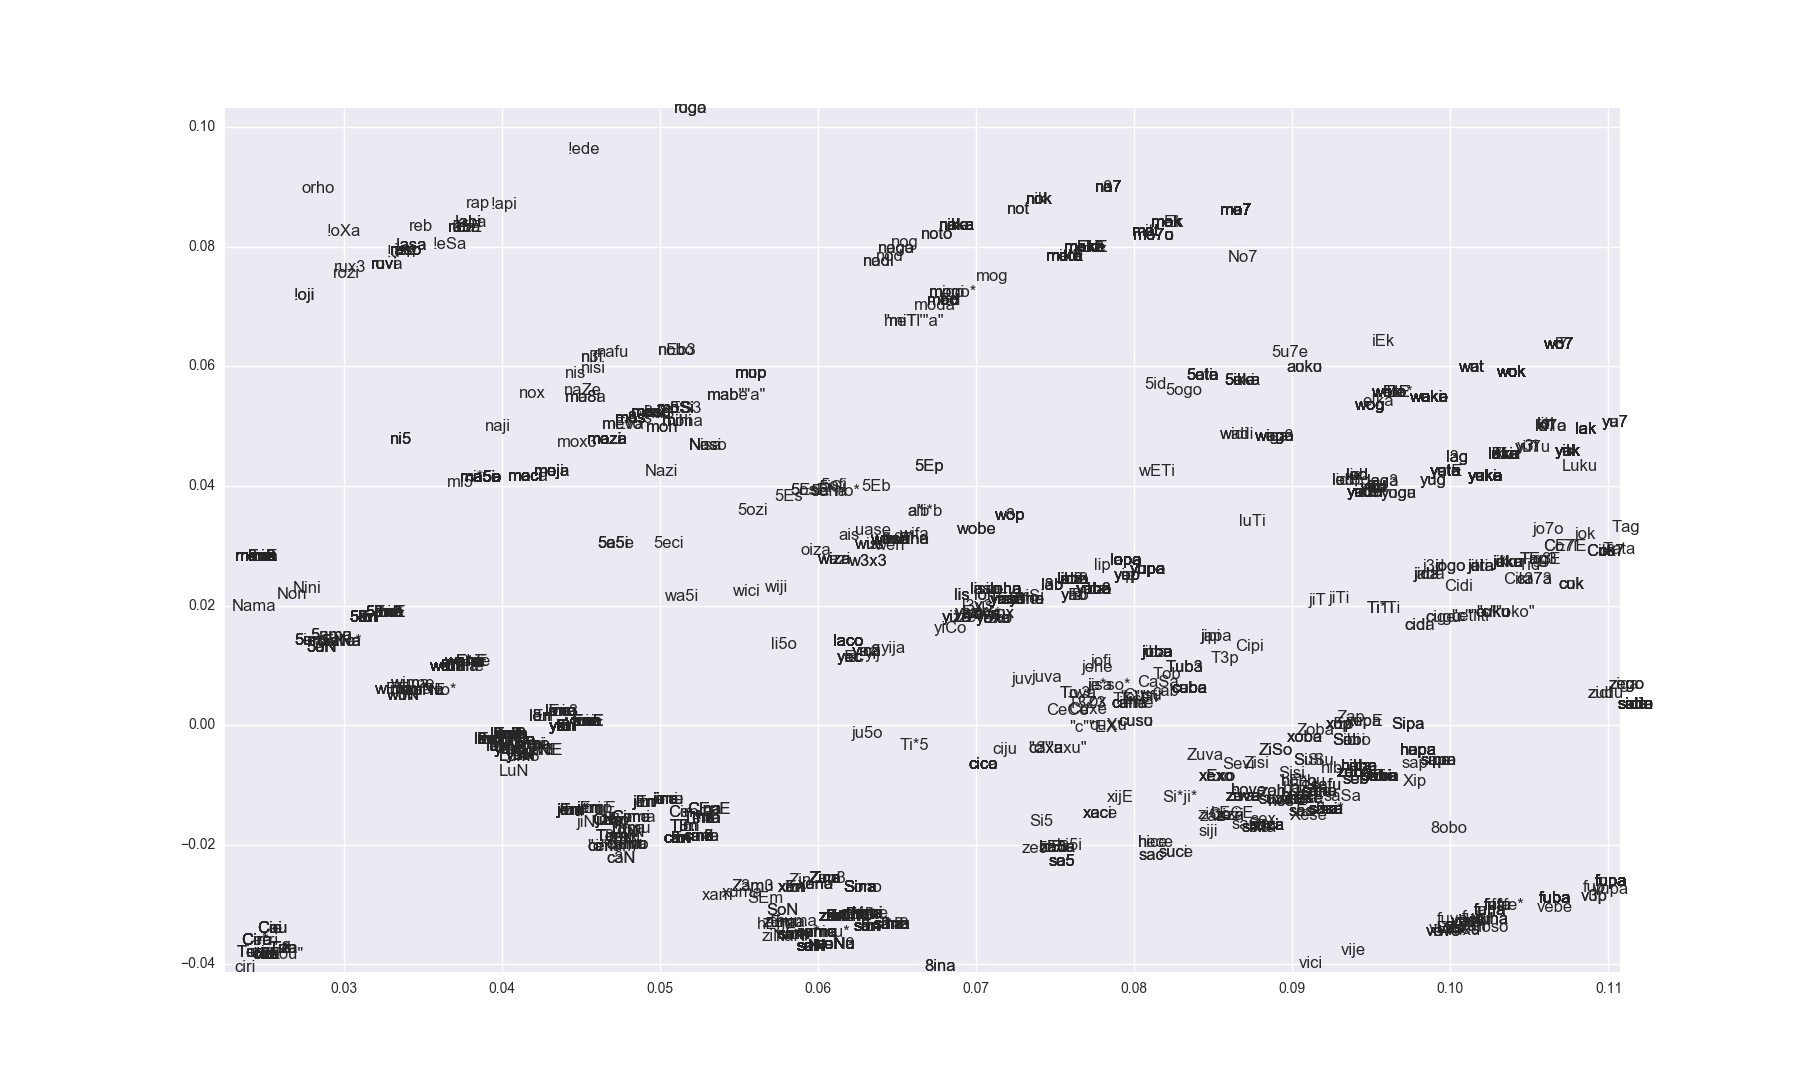
\includegraphics[width=\textwidth]{vae_phono_binary_asjp_subsample_words} 
   \caption{A detailed view on a subsample of ASJP embedded into $\mathcal{Z}$ after trained on the whole ASJP data set for 100 iterations. As can be seen, words accumulate in local subspaces with higher probability mass. Here, all words are contained in an area with shorter words that show simple CV syllable structures. Words that only differ in one distinctive feature are very close to each other, while linear dependencies over longer distances signify relationships over whole syllables that are exchanged.}
   \label{fig:vae_phono_binary_asjp_subsample_words}
\end{figure}

    
    \begin{figure}[ht] 
  \begin{subfigure}[b]{0.5\linewidth}
    \centering
    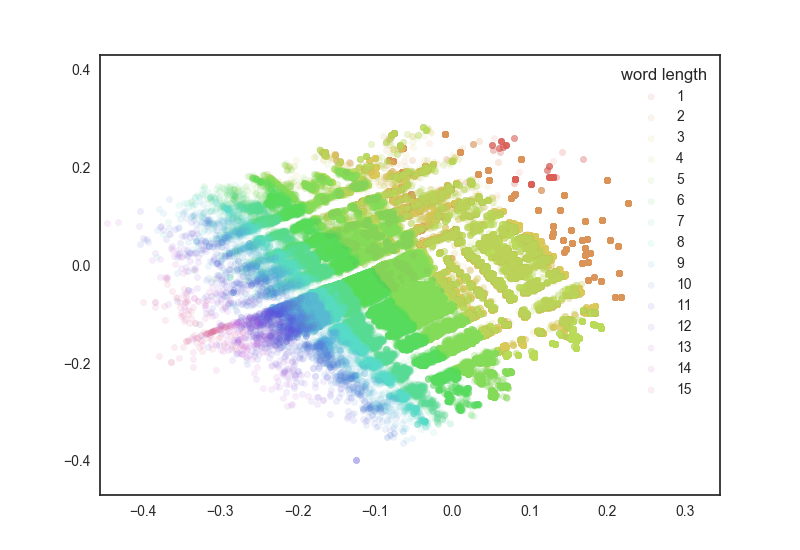
\includegraphics[width=\linewidth]{vae_phono_binary_wordLength} 
    \label{fig:vae_phono_binary_wordLength0} 
    \vspace{4ex}
  \end{subfigure}%% 
  \begin{subfigure}[b]{0.5\linewidth}
    \centering
    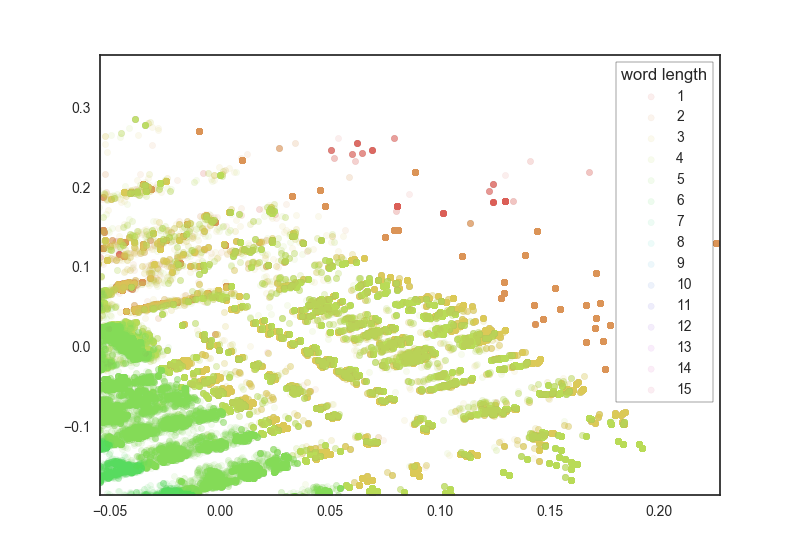
\includegraphics[width=\linewidth]{vae_phono_binary_wordLength_detail1} 
    \label{fig:vae_phono_binary_wordLength1} 
    \vspace{4ex}
  \end{subfigure} 
  \begin{subfigure}[b]{0.5\linewidth}
    \centering
    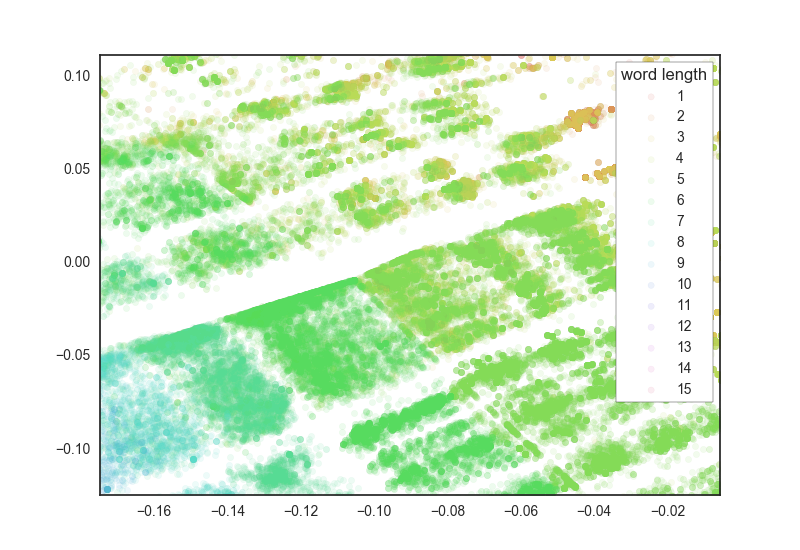
\includegraphics[width=\linewidth]{vae_phono_binary_wordLength_detail2} 
    \label{fig:vae_phono_binary_wordLength2} 
  \end{subfigure}%%
  \begin{subfigure}[b]{0.5\linewidth}
    \centering
    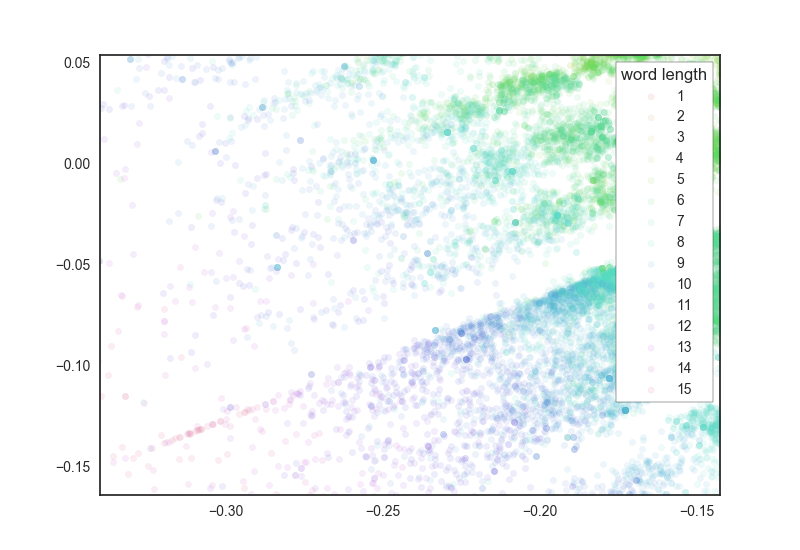
\includegraphics[width=\linewidth]{vae_phono_binary_wordLength_detail3} 
    \label{fig:vae_phono_binary_wordLength3} 
  \end{subfigure} 
  \caption{The ASJP data set embedded into $\mathcal{Z}$ after trained on it for 100 iterations, colored by word length. The model learns to cluster words according to their respective length, with more frequent word lengths located in subspaces with higher probability mass.}
  \label{fig:vae_phono_binary_wordLength} 
\end{figure}

    \begin{figure}[ht] 
  \begin{subfigure}[b]{0.5\linewidth}
    \centering
    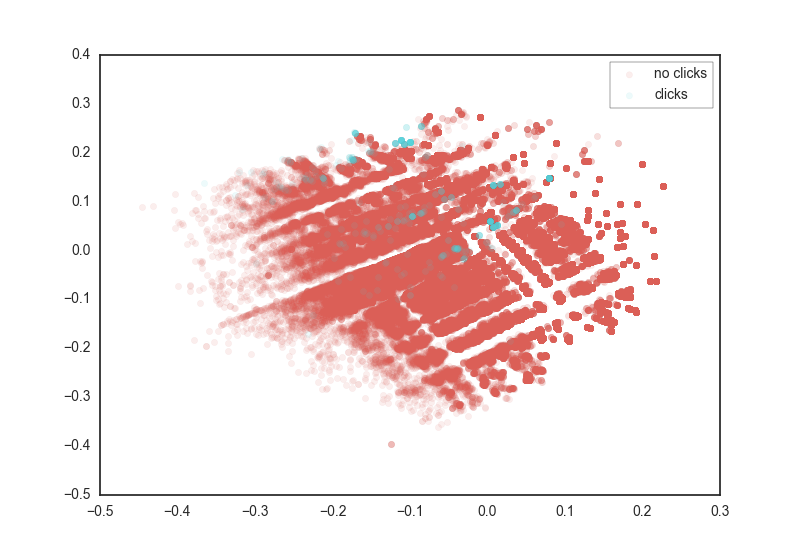
\includegraphics[width=\linewidth]{vae_phono_binary_clicks} 
    \label{fig:vae_phono_binary_features0} 
    \vspace{4ex}
  \end{subfigure}%% 
  \begin{subfigure}[b]{0.5\linewidth}
    \centering
    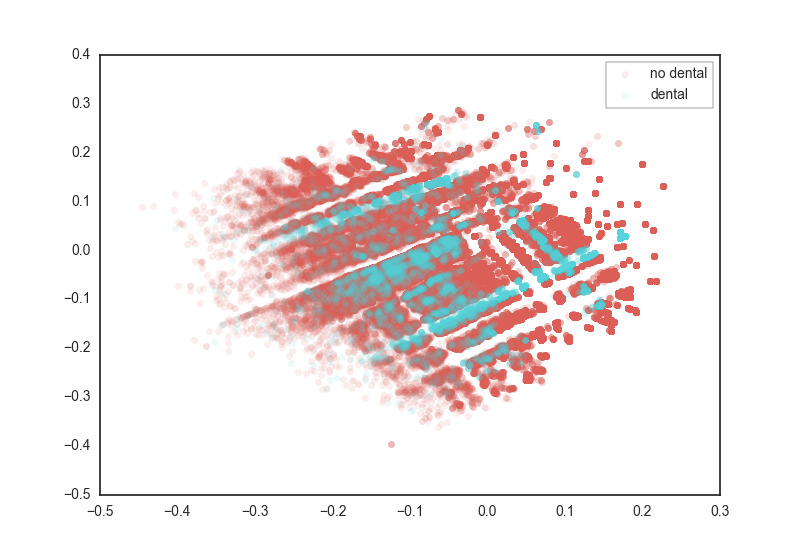
\includegraphics[width=\linewidth]{vae_phono_binary_dental} 
    \label{fig:vae_phono_binary_features1} 
    \vspace{4ex}
  \end{subfigure} 
  \begin{subfigure}[b]{0.5\linewidth}
    \centering
    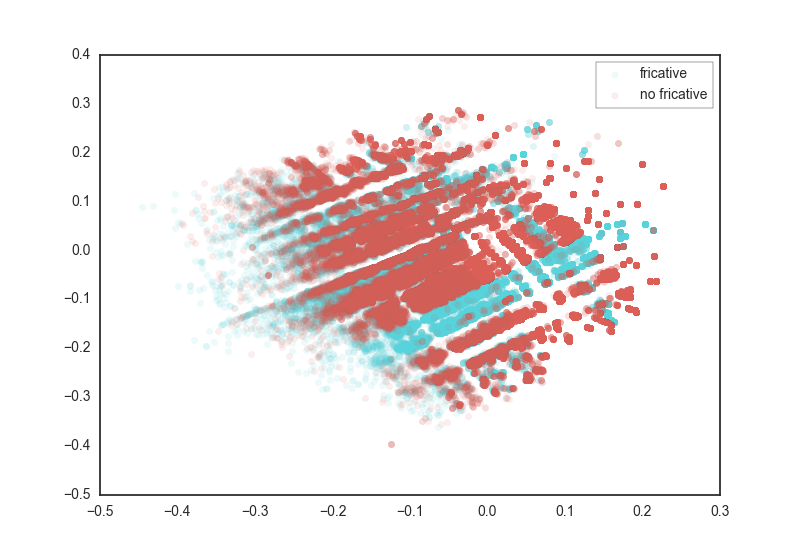
\includegraphics[width=\linewidth]{vae_phono_binary_fricative} 
    \label{fig:vae_phono_binary_features2} 
  \end{subfigure}%%
  \begin{subfigure}[b]{0.5\linewidth}
    \centering
    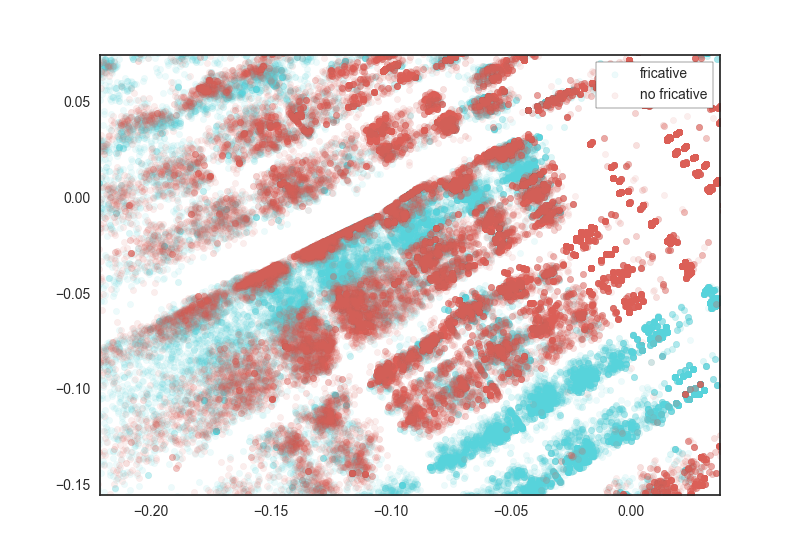
\includegraphics[width=\linewidth]{vae_phono_binary_fricative_detail1} 
    \label{fig:vae_phono_binary_feature3} 
  \end{subfigure} 
  \caption{The ASJP data set embedded into $\mathcal{Z}$ after trained on it for 100 iterations, colored by whether a given word has a phoneme with some specific distinctive feature. (top left) The model learns that clicks are highly unlikely to emerge evolutionary and hence assigns low probability mass to their respective subspace. (top right) The distribution of words with and without dentals. The linear dependencies are clearly visible. (bottom left) The distribution of words with and without fricatives. Again, it can be seen how they are linearly dependent of each other. (bottom right) A detailed view on the words with and without fricatives.}
  \label{fig:vae_phono_binary_features} 
\end{figure}

    \begin{figure}[ht] 
  \begin{subfigure}[b]{0.5\linewidth}
    \centering
    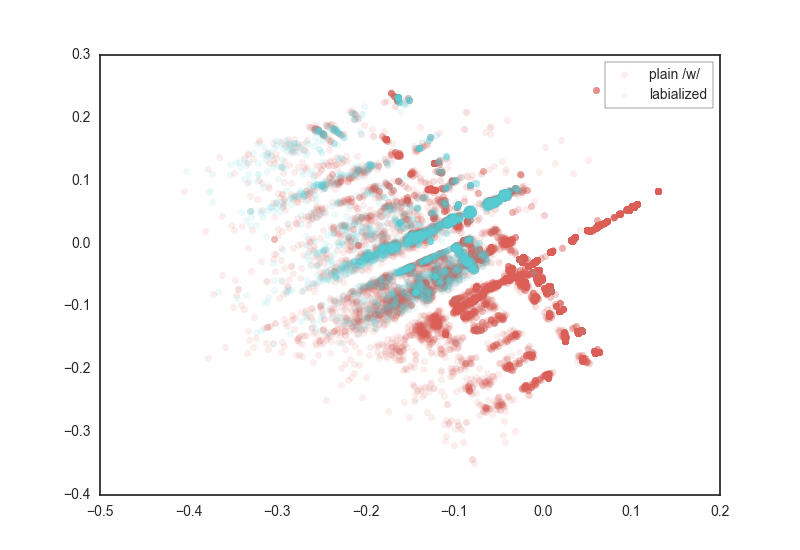
\includegraphics[width=\linewidth]{vae_phono_binary_orthofeature_labialized} 
    \label{fig:vae_phono_orthofeatures0} 
    \vspace{4ex}
  \end{subfigure}%% 
  \begin{subfigure}[b]{0.5\linewidth}
    \centering
    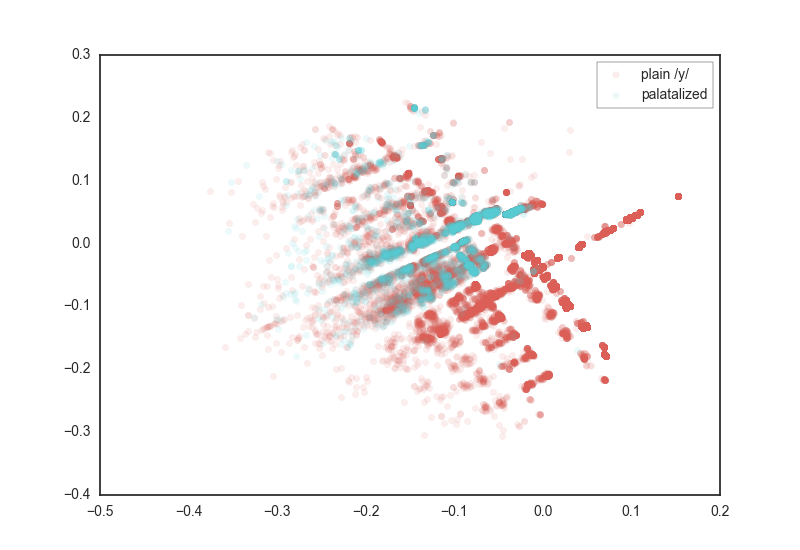
\includegraphics[width=\linewidth]{vae_phono_binary_orthofeature_palatalized} 
    \label{fig:vae_phono_orthofeatures1} 
    \vspace{4ex}
  \end{subfigure} 
  \begin{subfigure}[b]{0.5\linewidth}
    \centering
    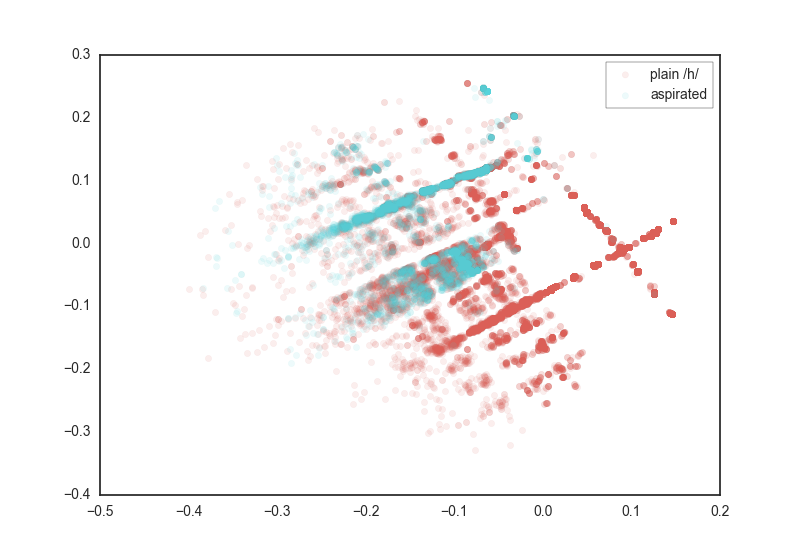
\includegraphics[width=\linewidth]{vae_phono_binary_orthofeature_aspirated} 
    \label{fig:vae_phono_orthofeatures2} 
  \end{subfigure}%%
  \begin{subfigure}[b]{0.5\linewidth}
    \centering
    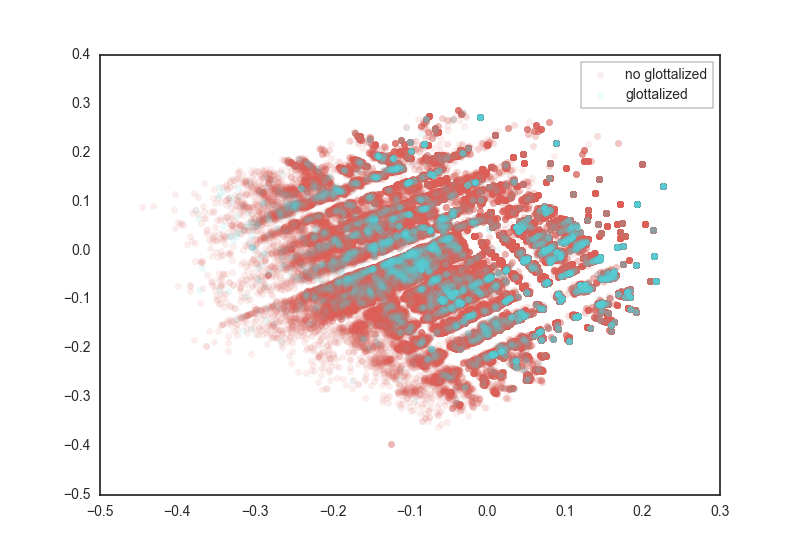
\includegraphics[width=\linewidth]{vae_phono_binary_orthofeature_glottalized} 
    \label{fig:vae_phono_orthofeatures3} 
  \end{subfigure} 
  \caption{The ASJP data set embedded into $\mathcal{Z}$ after trained on it for 100 iterations. Since the binary features ignore coarticulations as such and encode them as independent phonemes instead, the model might learn to distinguish them, given some underlying latent features. (top left) The distribution of words that contain plain /w/ versus words with proper labialization. If the model did not learn the difference, we would expect some uniform distributions over all words that contain /w/ in the input. However, we can clearly see that words with proper labialization are located in other subspaces than words with proper /w/. Moreover, we see that words with labialized phonemes show linear dependence. (top right) The distribution of words that contain plain /y/ versus words with proper palatalization. Again, we see a clear distinction between the two. (bottom left) The distribution of words that contain plain /h/ versus words with proper aspiration. Again, we see a clear distinction between the two. (bottom right) The distribution of words that contain glottalized sounds versus that of words without. As glottalization can cover both vowels and consonants, the distributions are spread over the whole population. However, we can see that glottalized sounds cluster at the bottom right, a subspace containing mostly mostly words with velar and uvular consonants.}
  \label{fig:vae_phono_orthofeatures} 
\end{figure}


 \begin{figure}[ht] 
  \begin{subfigure}[b]{0.5\linewidth}
    \centering
    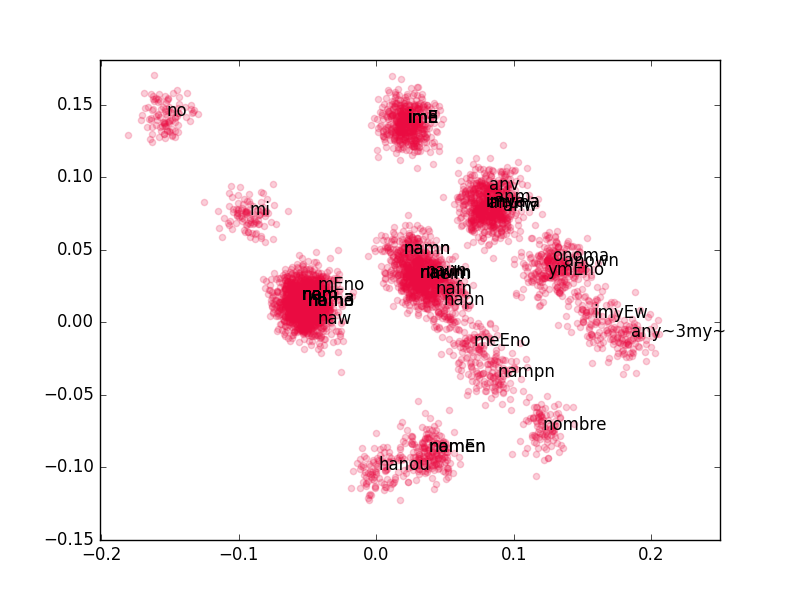
\includegraphics[width=\linewidth]{asjp_200_binary_singleConcept_posterior_name.png} 
    \label{fig:vae_phono_orthofeatures0} 
    \vspace{4ex}
  \end{subfigure}%% 
  \begin{subfigure}[b]{0.5\linewidth}
    \centering
    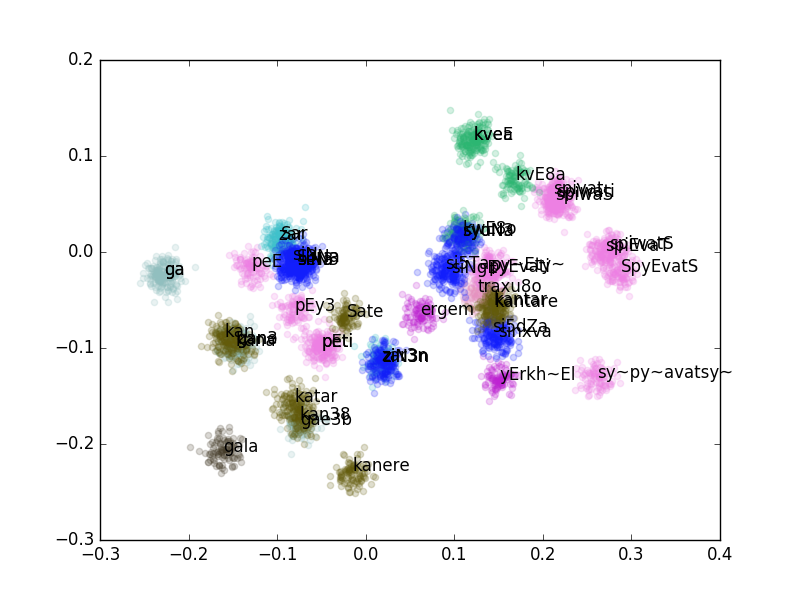
\includegraphics[width=\linewidth]{asjp_200_binary_singleConcept_posterior_sing.png} 
    \label{fig:vae_phono_orthofeatures1} 
    \vspace{4ex}
  \end{subfigure} 
  \begin{subfigure}[b]{0.5\linewidth}
    \centering
    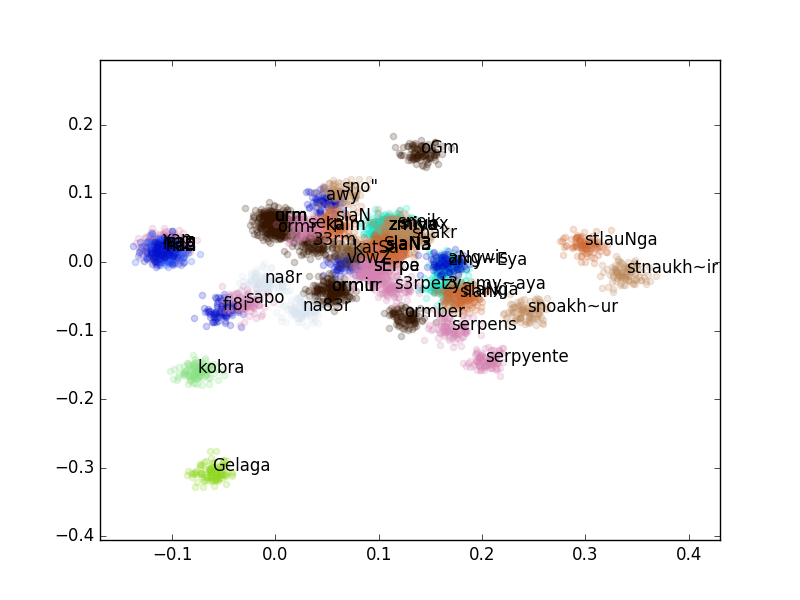
\includegraphics[width=\linewidth]{asjp_200_binary_singleConcept_posterior_snake.png} 
    \label{fig:vae_phono_orthofeatures2} 
  \end{subfigure}%%
  \begin{subfigure}[b]{0.5\linewidth}
    \centering
    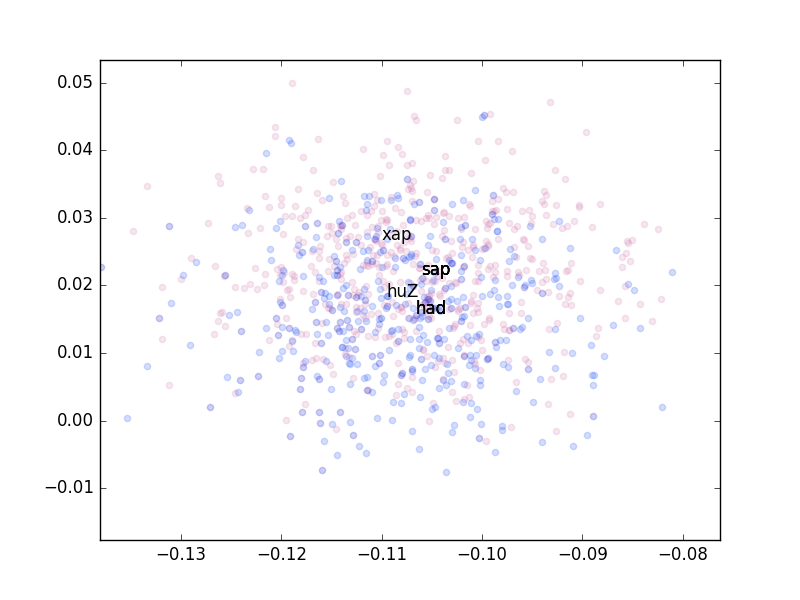
\includegraphics[width=\linewidth]{asjp_200_binary_singleConcept_posterior_snake_detail2.png} 
    \label{fig:vae_phono_orthofeatures3} 
  \end{subfigure} 
  \caption{The posterior distribution $P(z|X)$ with X being the IELex data with regards to the single semantic concepts. The model was trained on ASJP for 2000 iterations. Colors indicate the respective true cognate class. (top left) The posterior for the concept "name". As all words are cognates to each other, we see strong linear dependencies over the distribution. Also note that the embeddings are embedded into a latent continuum of word lengths, from the the top left to the bottom right. Moreover, the members of the left hand side clusters all start with consonants, while the members of the clusters on right hand side all start with vowels or approximants. (top right) The posterior for "sing". Again, cognates show stronger linear dependencies among each other. (bottom left) The posterior for "snake". The romance words (pink samples) show linear dependencies. (bottom right) A closer look on some words for "snake". As VAE-PT concentrates on clustering words with similar syllable structures, it tends to cluster words that share such similarities close to each other. Here, it overestimates the similarity between Slovak /had/ and Upper Sorbian /huZ/ on the one side and the words /sap/ (Bihari,Magahi,Urdu,Marathi) and /xap/ (Assamese) on the other.  }
  \label{fig:asjp_2000_binary_singleIELEXConcepts_posteriors} 
\end{figure}

\begin{figure}[h!] %  figure placement: here, top, bottom, or page
   \centering
   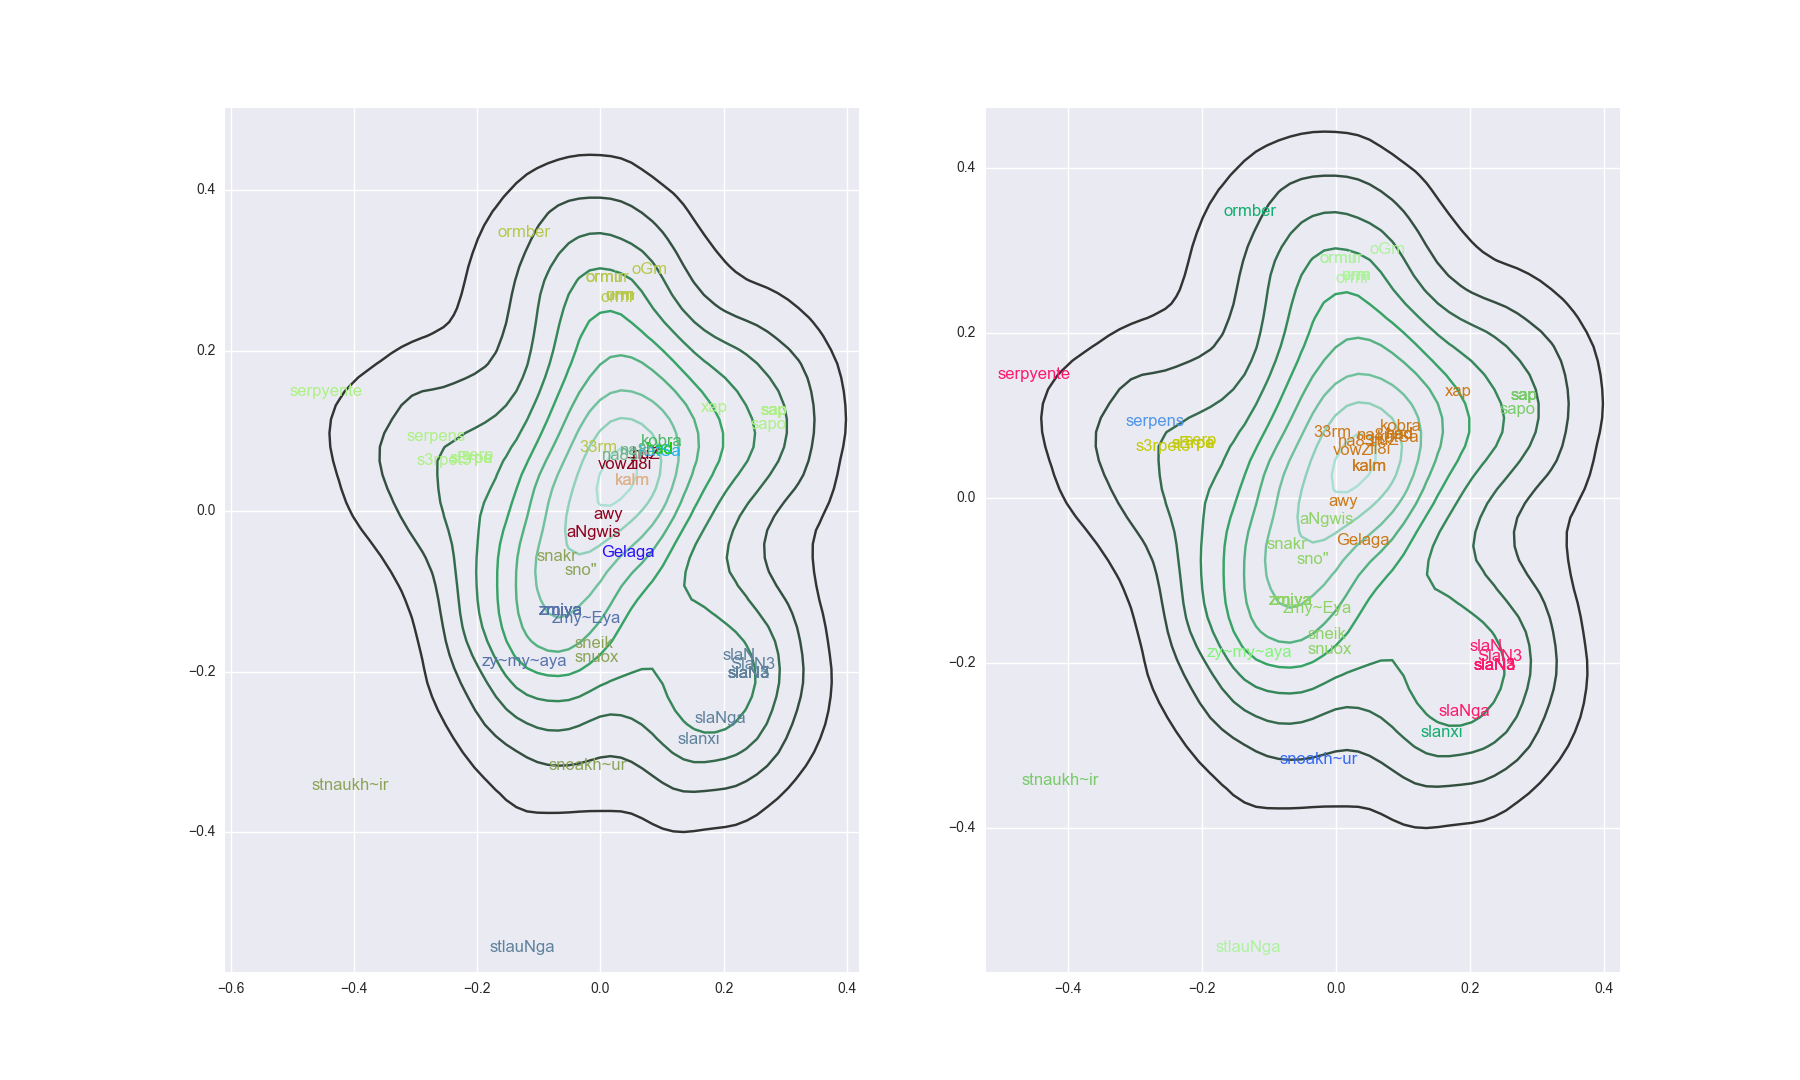
\includegraphics[width=\textwidth]{vae_c_snake} 
   \caption{VAE-C trained on the IELex data for "snake". The left plot shows true cognates classes, the right plot shows inferred labels. Cognates, as long as they appear similar, are clustered at some subspace of $\mathcal{Z}$. Words with low self-information, such was words with no inferred cognates, are seen as "noise" by the model and grouped close to each other at the center of the latent space.}
   \label{fig:vae_c_snake}
\end{figure}
\subsection{Grid Search over Model Parameters}

To explore the performances of VAE-C under different parameter settings, a grid search over the following parameters was performed:
\begin{itemize}
\item Phoneme vectorization:  \begin{itemize}
\item Dolgopolsky one hots \citep{dolgopolsky1986probabilistic,list2012sca}
\item SCA one hots \citep{list2012sca}
\item Binary ASJP phoneme features \citep{rama2016siamese})
\item Phoneme embeddings, as explored in \ref{Phoneme embeddings}, i.e. 20 embedding dimensions, CBOW, HS, trained on ASJP with all coarticulations removed. 
\end{itemize}
\item number of latent dimensions:  [10,20,50]
%\item intermediate dimensions of the encoding and decoding MLPs:  [100,200,500]
\item the standard deviation of the auxiliary noise $\sigma_{\epsilon}$: [0.1,0.01,0.001]
\end{itemize}
For all settings, the models were trained on a validation set of 10 concepts, which are randomly sampled from all IELex concepts beforehand. The models are trained for 4000 iterations. The encoding and decoding MLPs both have hidden layers of 1000 units. All words were zero-padded to a maximum length of 10 phonemes, following \citep{rama2016siamese}. The performance is measured in adjusted rand indices \citep{rand1971objective,hubert1985comparing}. 
Fig. \ref{fig:grid_search_boxplots} summarizes the results. The binary phoneme features outperform the word2vec phoneme embeddings, which perform nevertheless much better than the sound class one hot vectors. Also, the number of latent dimensions does not seem to influence the performance too much. While 10 latent dimensions slightly seem to outperform 20 and 50 in this grid search, higher-dimensional latent spaces are generally known to require more time to have a network converge, which could also be the case here - the 4000 iterations simply might not be enough for such higher-dimensional spaces. While we think that it is quite possible to improve the performance with an increased dimensionality of the latent space, as it should then be able to encode much more information in general, we do not think it is for practical value in our case. One the one hand, iterating a model over every semantic concept in the data set takes time. In our setup, 1000 iterations over one concept roughly took 20 seconds, varying by the number of latent dimensions and hidden dimensions of the encoding and decoding MLPs. Summed up for every single concept in the data and 4000 iterations for every such concept, it already took around 8 hours to perform that grid search from above. On the other hand, we do not expect the clustering to work efficiently in higher-dimensional space anymore anyway, as due to the the curse of dimensionality all points should then become more and more equidistant to each other, and thus clusters should be harder to identify. % While 10 dimensions slightly outperform 20, 10 dimensions show more variance, too. This might be an indicator to favor 20 dimensions.

The standard deviation of the auxiliary noise $\sigma_{\epsilon}$ also does not seem to influence the performance too much either. However, a rather high standard deviation seems to outperform the other configurations slightly. This might be due to the reasons discussed in section \ref{interpretation_of_z} - an increased auxiliary noise forces the network to learn more abstract features.

 \begin{figure}[h!] 
     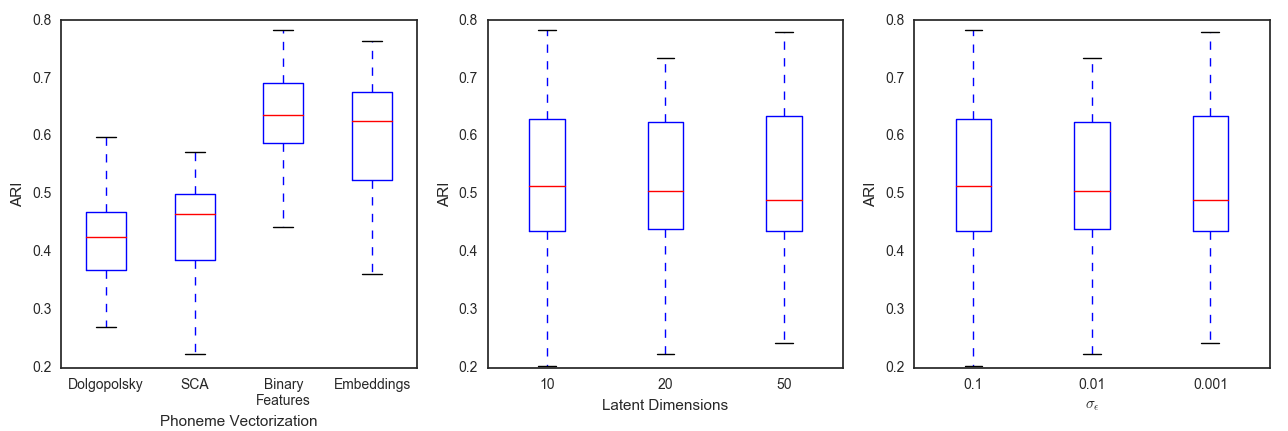
\includegraphics[width=\linewidth]{new_grid_search_boxplots} 
     \caption{The result of the grid search over several parameters of VAE-C, measured in adjusted rand indices. (left) The binary phoneme features outperform the phoneme embeddings. The sound class one hot vectors only show mediocre performance. (middle) the number of latent dimensions does not seem to influence the performance too much. An increased dimensionality shows slightly worse performance, but this might due to the network not having converged yet. (right) An increased auxiliary noise coincides with better performance over all model.}
    \label{fig:grid_search_boxplots} 
\end{figure}

\subsection{Performance on IELex}

VAE-C was then run on the remaining 197 semantic concepts on IELex with the parameters found optimal in the grid search above, i.e. binary phoneme features, 10 latent dimensions, 1000 intermediate dimensions and $\sigma_{\epsilon}= 0.1$. Fig. \ref{fig:boxplots_IELex} summarizes the results, measured in adjusted rand indices, adjusted mutual information \citep{vinh2010information}, cluster homogeneity, cluster completeness, v-measure \citep{rosenberg2007v} as well as pairwise precision, recall and F1-score.
The model indeed finds cognates and is far better than random labeling, but the overall performance is only mediocre, especially compared to LexStat (cf. table \ref{table:model_comparison})

\begin{table}
\begin{tabular}{l | rrrrrrrr}
\toprule
{} &       ARI &       AMI &         Homogeneity &        Completeness &         V-Measure &Precision&Recall&F1 \\  \hline
\midrule
VAE-C &  0.32 &  0.37 &  0.68 &  0.56 &  0.58 &  0.68 &  0.44 &  0.49 \\ 
LexStat & \textbf{0.58} & \textbf{0.71} & \textbf{0.99} & \textbf{0.91} &  \textbf{0.95} & \textbf{0.94} & \textbf{0.46} &  \textbf{0.62} \\
NLD-AP &  0.32 & 0.38 & 0.74 &0.57 & 0.60 & 0.71 & 0.42 & 0.48 \\
Random &  0.00 &  0.00 &  0.42 &  0.30 &  0.32 &  0.42 &  0.18 &  0.22 \\
\bottomrule
\end{tabular}
\caption{The performance of VAE-C compared to LexStat. NLD-AP uses Normalized Levenshtein Distances between IPA-annotated words as distance metric and Affinity Propagation as clustering algorithm. VAE-C performs only mediocre, but at least better than random labeling.}
\label{table:model_comparison} 
\end{table}

 \begin{figure}[h!] 
     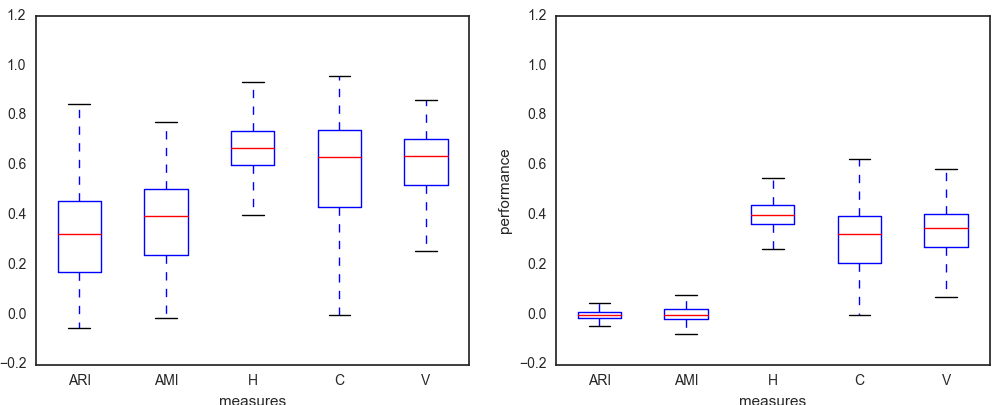
\includegraphics[width=\linewidth]{boxplots_IELex} 
     \caption{The performance of VAE-C on IELex, using the parameters obtained by the grid search (left), and random labeling (right). The measures are adjusted rand indices, adjusted mutual information, cluster homogeneity, cluster completeness and v-measure, as the harmonic mean of the latter two. The model learns to cluster similar words together, although the overall performance is mediocre.}
    \label{fig:boxplots_IELex} 
\end{figure}


%\subsection{Discussion}
%
%VAE-PT shows extraordinary performance in uncovering latent features. It can recognize the compositional structure of words, as it learns to form linear dependencies over distinctive phonological features, whole phonemes or even syllables. However, most information is encoded by such dependencies which is not suitable for flat clustering methods, where we expect that the location of a data point can be used to compare it with other data points. Although the smoothness assumption holds for VAE-PT, as we end up with clusters of very similar words, only a handful of actual cognates can be found in those. Following this, the performance of the model is quite bad, only slightly better than random labeling. 
%
%VAE-C however, performs much better than VAE-PT. It overfits to the training data, but by that encodes as much latent information as possible. Words with similar phonological structures cluster among each other. Although an increased auxiliary noise has its theoretical motivations, bigger values of $\sigma_{\epsilon}$ rather decrease the overall performance of the model. 
\section{Resume}

In this thesis, I have shown how recent tools from the emerging deep learning framework can be used for unsupervised cognate identification. Although the two models described here do not perform better than well-established methods on the task of cognate identification as such, they allow for great introspection on the compositional structure of words and the linear factors that create it. Especially when trained on a big corpus, the model can uncover very abstract features and hence could be a basis for more research on how and why certain words evolve differently than others. 
\section{Acknowledgements}
For training the phoneme embeddings, I used the word2vec implementations provided by the gensim package \citep{rehurek_lrec}. The Autoencoder was implemented with Keras \citep{chollet2015keras}, Tensorflow \citep{tensorflow2015-whitepaper} and theano \citep{2016arXiv160502688short}. For converting phonemes into the Dolgopolsky and SCA format, I used the lingpy library \citep{List2016e}. The clustering algorithms used here were provided by scikit-learn \citep{scikit-learn}. All code connected to this thesis can be found on my github \footnote{https://github.com/marlonbetz/BA}.
%\subsection{}


\bibliographystyle{apacite}
\bibliography{references}
\end{document}  